%%%% Шаблон ВКР <<SPbPU-student-thesis-template>>  %%%%
%%
%%   Создан на основе глубокой переработки шаблона российских кандидатских и докторских диссертаций [1]. 
%%   
%%   Полный список различий может быть получен командами git.
%%   Лист авторов-составителей расположен в README.md файле.
%%   Подробные инструкции по использованию в [1,2].
%%   
%%   Рекомендуем установить TeX Live + TeXstudio
%%   <<Стандартная>> компиляция 2-3 РАЗА с помощью pdflatex + biber (для библиографии)     
%%  
%%%% Student thesis template <<SPbPU-student-thesis-template>> %%%%
%%
%%   Created on the basis of deepl modifification of the Russian candidate and doctorate thesis template [1]. 
%%   
%%   Full list of differences can be achieved by git commands.
%%   List of template authors can be seen in the README.md file.
%%   Detailed instructions of usage, see, please in [1,2].
%%     
%%   [1] github.com/AndreyAkinshin/Russian-Phd-LaTeX-Dissertation-Template 
%%   [2] Author_guide_SPBPU-student-thesis-template.pdf
%%   
%%   It is recommended to install TeX Live + TeXstudio   
%%   Default compilation 2-3 TIMES with pdflatex + biber (for the bibliography)
%%  
\input{template_settings/ch_preamble} % лучше не редактировать / please, keep unmodified

\setcounter{docType}{1} % лучше не редактировать / please, keep unmodified

%%%% Настройки автора / Author settings
%% 
\input{my_folder/my_settings} % добавляем свои команды / update your commands


\begin{document} % начало документа


%%% Внесите свои данные - Input your data
%%
%%
\newcommand{\Author}{Д.А.\,Кучмин} % И.О. Фамилия автора 
\newcommand{\AuthorFull}{Кучмин Дмитрий Алексеевич} % Фамилия Имя Отчество автора
\newcommand{\AuthorFullDat}{Кучмину Дмитрию Алексеевичу} % Фамилия Имя Отчество автора в дательном падеже (Кому? Студенту...)
\newcommand{\AuthorFullVin}{Кучмина Дмитрия Алексеевича} % в винительном падеже (Кого? что?  Програмиста ...)
\newcommand{\AuthorPhone}{+7-931-244-14-97} % номер телефорна автора для оперативной связи  
\newcommand{\Supervisor}{В.М.\,Ицыксон} % И. О. Фамилия научного руководителя
\newcommand{\SupervisorFull}{Ицыксон Владимир Михайлович} % Фамилия Имя Отчество научного руководителя
\newcommand{\SupervisorVin}{В.М.\,Ицыксона} % И. О. Фамилия научного руководителя  в винительном падеже (Кого? что? Руководителя ...)
\newcommand{\SupervisorJob}{к.т.н} %
\newcommand{\SupervisorJobVin}{должность} % в винительном падеже (Кого? что?  Програмиста ...)
\newcommand{\SupervisorDegree}{доцент} %
\newcommand{\SupervisorTitle}{} % звание
%%
%%
%Руководитель, утверждающий задание
\newcommand{\Head}{В.М.\,Ицыксон} % И. О. Фамилия руководителя подразделения (руководителя ОП)
\newcommand{\HeadDegree}{Директор ВШИСиСТ}% Только должность:
%Руководитель %ОП 
%Заведующий % кафедрой
%Директор % Высшей школы
%Зам. директора
\newcommand{\HeadDep}{} % заменить на краткую аббревиатуру подразделения или оставить пустым, если утверждает руководитель ОП

%%% Руководитель, принимающий заявление
\newcommand{\HeadAp}{И.О.\,Фамилия} % И. О. Фамилия руководителя подразделения (руководителя ОП)
\newcommand{\HeadApDegree}{Должность руководителя}% Только должность:   
%Руководитель ОП 
%Заведующий кафедрой
%Директор Высшей школы
\newcommand{\HeadApDep}{O} % заменить на краткую аббревиатуру подразделения или оставить пустым, если утверждает руководитель ОП
%%% Консультант по нормоконтролю
\newcommand{\ConsultantNorm}{А.Г.\,Новопашенный} % И. О. Фамилия консультанта по нормоконтролю. ТОЛЬКО из числа ППС!
\newcommand{\ConsultantNormDegree}{должность, степень} %   
%%% Первый консультант
\newcommand{\ConsultantExtraFull}{Фамилия Имя Отчетство} % Фамилия Имя Отчетство дополнительного консультанта 
\newcommand{\ConsultantExtra}{И.О.\,Фамилия} % И. О. Фамилия дополнительного консультанта 
\newcommand{\ConsultantExtraDegree}{должность, степень} % 
\newcommand{\ConsultantExtraVin}{И.О.\,Фамилию} % И. О. Фамилия дополнительного консультанта в винительном падеже (Кого? что? Руководителя ...)
\newcommand{\ConsultantExtraDegreeVin}{должность, степень} %  в винительном падеже (Кого? что? Руководителя ...)
%%% Второй консультант
\newcommand{\ConsultantExtraTwoFull}{Фамилия Имя Отчетство} % Фамилия Имя Отчетство дополнительного консультанта 
\newcommand{\ConsultantExtraTwo}{И.О.\,Фамилия} % И. О. Фамилия дополнительного консультанта 
\newcommand{\ConsultantExtraTwoDegree}{должность, степень} % 
\newcommand{\ConsultantExtraTwoVin}{И.О.\,Фамилию} % И. О. Фамилия дополнительного консультанта в винительном падеже (Кого? что? Руководителя ...)
\newcommand{\ConsultantExtraTwoDegreeVin}{должность, степень} %  в винительном падеже (Кого? что? Руководителя ...)
\newcommand{\Reviewer}{И.О.\,Фамилия} % И. О. Фамилия резензента. Обязателен только для магистров.
\newcommand{\ReviewerDegree}{должность, степень} % 
%%
%%
\renewcommand{\thesisTitle}{Интерактивный визуализатор моделей программ}
\newcommand{\thesisDegree}{бакалавра}% дипломный проект, дипломная работа, магистерская диссертация %c 2020
\newcommand{\thesisTitleEn}{Interactive visualizer of program models} %2020
\newcommand{\thesisDeadline}{16.06.2022}
\newcommand{\thesisStartDate}{06.05.2022}
\newcommand{\thesisYear}{2022}
%%
%%
\newcommand{\group}{3530901/80101} % заменить вместо N номер группы
\newcommand{\thesisSpecialtyCode}{09.03.01}% код направления подготовки
\newcommand{\thesisSpecialtyTitle}{<<Информатика и вычислительная техника>>} % наименование направления/специальности
\newcommand{\thesisOPPostfix}{01} % последние цифры кода образовательной программы (после <<_>>)
\newcommand{\thesisOPTitle}{Разработка компьютерных систем}% наименование образовательной программы
%%
%%
\newcommand{\institute}{
Институт компьютерных наук и~технологий
%Гуманитарный институт
%Инженерно-строительный институт
%Институт биомедицинских систем и технологий
%Институт металлургии, машиностроения и транспорта
%Институт передовых производственных технологий
%Институт прикладной математики и механики
%Институт физики, нанотехнологий и телекоммуникаций
%Институт физической культуры, спорта и туризма
%Институт энергетики и транспортных систем
%Институт промышленного менеджмента, экономики и торговли
}%
%%
%%




%%% Задание ключевых слов и аннотации
%%
%%
%% Ключевых слов от 3 до 5 слов или словосочетаний в именительном падеже именительном падеже множественного числа (или в единственном числе, если нет другой формы) по правилам русского языка!!!
%%
%%
\newcommand{\keywordsRu}{статический анализ, модели программ, Java, верификация и анализ программ, динамическая визуализация} % ВВЕДИТЕ ключевые слова по-русски
%%
%%
\newcommand{\keywordsEn}{static analysis, program models, Java, program verification and analysis, dynamic visualization} % ВВЕДИТЕ ключевые слова по-английски
%%
%%
%% Реферат ОТ 1000 ДО 1500 знаков на русский или английский текст
%%
%Реферат должен содержать:
%- предмет, тему, цель ВКР;
%- метод или методологию проведения ВКР:
%- результаты ВКР:
%- область применения результатов ВКР;
%- выводы.

\newcommand{\abstractRu}{Данная работа представляет собой разработку интерактивного визуализатора моделей программ, который упростит подачу материала студентам и поможет разобраться в устройстве абстрактного синтаксического дерева, графа потока управления, графа зависимости по данным, графа зависимости программы, абстрактного семантического графа и представления на основе однократного статического присваивания.\\
\indentРезультатом работы является клиент-серверное приложение, визуализирующее все вышеупомянутые модели. Приложение поддерживает программный код, написанный на Java.} % ВВЕДИТЕ текст аннотации по-русски
%%
%%
\newcommand{\abstractEn}{This work is the development of an interactive visualizer of program models that will simplify the presentation of material to students and help to understand the structure of an abstract syntax tree, a control flow graph, a data dependency graph, a program dependency graph, an abstract semantic graph, and a representation based on a single static assignment.\\
\indent The result of the work is a client-server application that visualizes all the above models. The application supports program code written in Java.} % ВВЕДИТЕ текст аннотации по-английски


%%% РАЗДЕЛ ДЛЯ ОФОРМЛЕНИЯ ПРАКТИКИ
%Место прохождения практики
\newcommand{\PracticeType}{Отчет о прохождении % 
	%стационарной производственной (технологической (проектно-технологической)) %
	такой-то % тип и вид ЗАМЕНИТЬ
	практики}

\newcommand{\Workplace}{СПбПУ, ИКНТ, ВШИСиСТ} % TODO Rename this variable

% Даты начала/окончания
\newcommand{\PracticeStartDate}{%
дд.мм.гггг%
%	22.06.2020
}%
\newcommand{\PracticeEndDate}{%
	дд.мм.гггг%
%	18.07.2020%
}%
%%

\newcommand{\School}{
	Название высшей школы
%	Высшая школа интеллектуальных систем и~суперкомпьютерных~технологий 
}
\newcommand{\practiceTitle}{Тема практики}


%% ВНИМАНИЕ! Необходимо либо заменить текст аннотации (ключевых слов) на русском и английском, либо удалить там весь текст, иначе в свойства pdf-отчета по практике пойдет шаблонный текст.

%%% Не меняем дальнейшую часть - Do not modify the rest part
%%
%%
%%
%%
\ifnumequal{\value{docType}}{1}{% Если ВКР, то...
	\newcommand{\DocType}{Выпускная квалификационная работа}
	\newcommand{\pdfDocType}{\DocType~(\thesisDegree)} %задаём метаданные pdf файла
	\newcommand{\pdfTitle}{\thesisTitle}
}{% Иначе 
	\newcommand{\DocType}{\PracticeType}
	\newcommand{\pdfDocType}{\DocType} %задаём метаданные pdf файла
	\newcommand{\pdfTitle}{\practiceTitle}
}%
\newcommand{\HeadTitle}{\HeadDegree~\HeadDep}
\newcommand{\HeadApTitle}{\HeadApDegree~\HeadApDep}
\newcommand{\thesisOPCode}{\thesisSpecialtyCode\_\thesisOPPostfix}% код образовательной программы
\newcommand{\thesisSpecialtyCodeAndTitle}{\thesisSpecialtyCode~\thesisSpecialtyTitle}% Код и наименование направления/специальности
\newcommand{\thesisOPCodeAndTitle}{\thesisOPCode~\thesisOPTitle} % код и наименование образовательной программы
%%
%%
\hypersetup{%часть болка hypesetup в style
		pdftitle={\pdfTitle},    % Заголовок pdf-файла
		pdfauthor={\AuthorFull},    % Автор
		pdfsubject={\pdfDocType. Шифр и наименование направления подготовки: \thesisSpecialtyCodeAndTitle. \abstractRu},      % Тема
		pdfcreator={LaTeX, SPbPU-student-thesis-template},     % Приложение-создатель
%		pdfproducer={},  % Производитель, Производитель PDF % будет выставлена автоматически
		pdfkeywords={\keywordsRu}
}
%%
%%
%% вспомогательные команды
\newcommand{\firef}[1]{рис.\ref{#1}} %figure reference
\newcommand{\taref}[1]{табл.\ref{#1}}	%table reference
%%
%%
%% Архивный вариант задания ключевых слов, аннотации и благодарностей 
% Too hard to export data from the environment to pdf-info
% https://tex.stackexchange.com/questions/184503/collecting-contents-of-environment-and-store-them-for-later-retrieval
%заменить NewEnviron на newenvironment для распознавания команды в TexStudio
%\NewEnviron{keywordsRu}{\noindent\MakeUppercase{\BODY}}
%\NewEnviron{keywordsEn}{\noindent\MakeUppercase{\BODY}}
%\newenvironment{abstractRu}{}{}
%\newenvironment{abstractEn}{}{}
%\newenvironment{acknowledgementsRu}{\par{\normalfont \acknowledgements.}}{}
%\newenvironment{acknowledgementsEn}{\par{\normalfont \acknowledgementsENG.}}{}


%%% Переопределение именований %%% Не меняем - Do not modify
%\newcommand{\Ministry}{Минобрнауки России} 
\newcommand{\Ministry}{Министерство науки и высшего образования Российской~Федерации} %с 2020
\newcommand{\SPbPU}{Санкт-Петербургский политехнический университет Петра~Великого}
\newcommand{\SPbPUOfficialPrefix}{Федеральное государственное автономное образовательное учреждение высшего образования}
\newcommand{\SPbPUOfficialShort}{ФГАОУ~ВО~<<СПбПУ>>}
%% Пробел между И. О. не допускается.
\renewcommand{\alsoname}{см. также}
\renewcommand{\seename}{см.}
\renewcommand{\headtoname}{вх.}
\renewcommand{\ccname}{исх.}
\renewcommand{\enclname}{вкл.}
\renewcommand{\pagename}{Pages}
\renewcommand{\partname}{Часть}
\renewcommand{\abstractname}{\textbf{Аннотация}}
\newcommand{\abstractnameENG}{\textbf{Annotation}}
\newcommand{\keywords}{\textbf{Ключевые слова}}
\newcommand{\keywordsENG}{\textbf{Keywords}}
\newcommand{\acknowledgements}{\textbf{Благодарности}}
\newcommand{\acknowledgementsENG}{\textbf{Acknowledgements}}
\renewcommand{\contentsname}{Content} % 
%\renewcommand{\contentsname}{Содержание} % (ГОСТ Р 7.0.11-2011, 4)
%\renewcommand{\contentsname}{Оглавление} % (ГОСТ Р 7.0.11-2011, 4)
\renewcommand{\figurename}{Рис.} % Стиль СПбПУ
%\renewcommand{\figurename}{Рисунок} % (ГОСТ Р 7.0.11-2011, 5.3.9)
\renewcommand{\tablename}{Таблица} % (ГОСТ Р 7.0.11-2011, 5.3.10)
%\renewcommand{\indexname}{Предметный указатель}
\renewcommand{\listfigurename}{Список рисунков}
\renewcommand{\listtablename}{Список таблиц}
\renewcommand{\refname}{\fullbibtitle}
\renewcommand{\bibname}{\fullbibtitle}

\newcommand{\chapterEnTitle}{Сhapter title} % <- input the English title here (only once!) 
\newcommand{\chapterRuTitle}{Название главы}          % <- введите 
\newcommand{\sectionEnTitle}{Section title} %<- input subparagraph title in english
\newcommand{\sectionRuTitle}{Название подраздела} % <- введите название подраздела по-русски
\newcommand{\subsectionEnTitle}{Subsection title} % - input subsection title in english
\newcommand{\subsectionRuTitle}{Название параграфа} % <- введите название параграфа по-русски
\newcommand{\subsubsectionEnTitle}{Subsubsection title} % <- input subparagraph title in english
\newcommand{\subsubsectionRuTitle}{Название подпараграфа} % <- введите название подпараграфа по-русски % Заполнить сведения, 
										 % в т.ч. ключевые слова и аннотацию.

%%% Титульник ВКР / Thesis title 
%%
%% добавить лист в pdf-навигацию 
%% add to pdf navigation menu
%%
\pdfbookmark[-1]{\pdfTitle}{tit}
%%
\thispagestyle{empty}%
\makeatletter
\newgeometry{top=2cm,bottom=2cm,left=3cm,right=1cm,headsep=0cm,footskip=0cm}
\savegeometry{NoFoot}%
\makeatother


%%% Распечатать версию документа / Print document version
%%
%\begin{flushright}
%	\vspace{0pt plus0.1fill}
%	\boxed{\small
%		\begin{tabular}{r} 
%			\textbf{Пример ВКР <<SPbPU-student-thesis-template>>.} %\\ % перенос на новую строку
%			\textbf{Версия от \today % \; время:  \currenttime. % время версии
%			}
%		\end{tabular}
%	} %end boxed
%	\vspace*{-5pt} % раскомментировать, если не хватает места
%	\vspace{0pt plus0.1fill} % раскоментировать, если хватает места
%\end{flushright}

{\centering%
	\Ministry\\
	\SPbPU\\
	{%\bfseries %2020 - указание на изменения, которые могут быть введены в 2020 году
		\institute}
\par}%


\vspace{0pt plus1fill} %число перед fill = кратность относительно некоторого расстояния fill, кусками которого заполнены пустые места


\noindent
\begin{minipage}{\linewidth}
	\vspace{\mfloatsep} % интервал 
	\begin{tabularx}{\linewidth}{Xl}
	&Работа допущена к защите     \\
	&\HeadTitle     \\			
	&\underline{\hspace*{0.1\textheight}} \Head     \\
	&<<\underline{\hspace*{0.05\textheight}}>> \underline{\hspace*{0.1\textheight}} \thesisYear~г.  \\ 
	\end{tabularx}
	\vspace{\mfloatsep} % интервал 	
\end{minipage}


\vspace{0pt plus2fill} %


{\centering%
	
	\MakeUppercase{\bfseries{}\DocType} \\ 
	\MakeUppercase{\thesisDegree}%


%\intervalS% %ОБЯЗАТЕЛЬНО ДОБАВИТЬ ОТСТУП, ЕСЛИ ХВАТАЕТ МЕСТА
{\centering%
	\MakeUppercase{\bfseries{\thesisTitle}}}%

}\par%
%\noindent
{\centering
%\intervalS% %ОБЯЗАТЕЛЬНО ДОБАВИТЬ ОТСТУП, ЕСЛИ ХВАТАЕТ МЕСТА
%по специальности % для специалистов
    	по направлению \thesisSpecialtyCodeAndTitle{}\\% для бакалавров и магистров 
%\noindent Направленность  % для специалистов
по образовательной программе\\


\thesisOPCodeAndTitle % для бакалавров и магистров
% Лучше по~профилю, но что делать, так составили Положение
\par%
}\par%




\vspace{4mm plus2fill}%

\noindent
\begin{tabularx}{\linewidth}{lXl}
	Выполнил              &	   &             \\
	студент гр.~\group     &    & \Author     \\[\mfloatsep]

	Руководитель 	    	  &    &             \\
	\SupervisorJob,	    	  &    &             \\
	\SupervisorDegree, \SupervisorTitle 	  &  \emph{<подпись>}  & \Supervisor \\[\mfloatsep]
	
	Консультант  &    &  \\   	
	по нормоконтролю                          &  \emph{<подпись>}  & \ConsultantNorm  % обязателен
\end{tabularx} %


%
\vspace{0pt plus4fill}% 


\begin{center}%
Санкт-Петербург\\
\thesisYear
\end{center}%
\restoregeometry
\newpage					 % Титульный лист
										 % Убираем footnotes, консультанта, если нет

%%%% Начало оформления заголовка - оставить без изменений !!! %%%%
\input{my_folder/task_settings}	% настройки - начало 
	
				{%\normalfont %2020
						\MakeUppercase{\SPbPU}}\\
				\institute

\par}\intervalS% завершает input

				\noindent
				\begin{minipage}{\linewidth}
				\vspace{\mfloatsep} % интервал 	
				\begin{tabularx}{\linewidth}{Xl}
					&УТВЕРЖДАЮ      \\
					&\HeadTitle     \\			
					&\underline{\hspace*{0.1\textheight}} \Head     \\
					&<<\underline{\hspace*{0.05\textheight}}>> \underline{\hspace*{0.1\textheight}} \thesisYear г.  \\  
				\end{tabularx}
				\vspace{\mfloatsep} % интервал 	
				\end{minipage}

\intervalS{\centering\bfseries%

				ЗАДАНИЕ\\
				на выполнение %с 2020 года 
				%по выполнению % до 2020 года
				выпускной квалификационной работы


\intervalS\normalfont%

				студенту \uline{\AuthorFullDat{} гр.~\group}


\par}\intervalS%
%%%%
%%%% Конец оформления заголовка  %%%%
 	
	
	
\begin{enumerate}[1.]
	\item Тема работы: {\expandafter \ulined \thesisTitle.}
	%\item Тема работы (на английском языке): \uline{\thesisTitleEn.} % вероятно после 2021 года
	\item Срок сдачи студентом законченной работы: \uline{\thesisDeadline.} 
	%\item Исходные данные по работе: \uline{статистические данные с сайта \cite{gosstat}, а также из репозитория \cite{uci}; основным источником литературы является монография \cite{Book} и статья \cite{Article}.}%
	%\printbibliographyTask % печать списка источников % КОММЕНТИРУЕМ ЕСЛИ НЕ ИСПОЛЬЗУЕТСЯ
	% В СЛУЧАЕ, ЕСЛИ НЕ ИСПОЛЬЗУЕТСЯ МОЖНО ТАКЖЕ ЗАЙТИ В setup.tex и закомментировать \vspace{-0.28\curtextsize}
	\item Содержание работы (перечень подлежащих разработке вопросов):
	\begin{enumerate}[label=\theenumi\arabic*.]
		\item Изучение предметной области и аналогов.
		\item Выбор используемых технологий.
		\item Разработка интерактивного визуализатора моделей программ.
		\item Тестирование интерактивного визуализатора моделей программ.
	\end{enumerate}
	%\item Перечень графического материала (с указанием обязательных чертежей): 
	%\begin{enumerate}[label=\theenumi\arabic*.]
	%	\item Схема работы метода/алгоритма.
	%	\item Архитектура разработанной программы/библиотеки.
	%\end{enumerate}	
	%	\item Консультанты по работе\footnote{Подпись консультанта по нормоконтролю пока не требуется. Назначается всем по умолчанию.}:
	%	\begin{enumerate}[label=\theenumi\arabic*.] 
	%	\item  \uline{\emakefirstuc{\ConsultantExtraDegree}, \ConsultantExtra.} % закомментировать при необходимости, идёт первый по порядку.
	%	\item \uline{\emakefirstuc{\ConsultantNormDegree}, \ConsultantNorm{} (нормоконтроль).} %	Обязателен для всех студентов
	%\end{enumerate}
		\item Дата выдачи задания: \uline{\thesisStartDate.}
\end{enumerate}

\intervalS%можно удалить пробел

Руководитель ВКР \uline{\hspace*{0.1\textheight} \Supervisor}


%\intervalS%можно удалить пробел

%Консультант\footnote{В случае, если есть консультант, отличный от консультанта по нормоконтролю.}  \uline{\hspace*{0.1\textheight}\ConsultantExtra}


%\intervalS%можно удалить пробел

%Консультант по нормоконтролю \uline{\hspace*{0.1\textheight} \ConsultantNorm}%ПОКА НЕ ТРЕБУЕТСЯ, Т.К. ОН У ВСЕХ ПО УМОЛЧАНИЮ

Задание принял к исполнению \uline{\thesisStartDate}

%\intervalS%можно удалить пробел

Студент \uline{\hspace*{0.1\textheight}  \Author}



\input{my_folder/task_settings_restore}	% настройки - конец					 % Задание 
										 % Для сдачи в высшую школу компилируем двухсторонний My_task.tex 
										 % После подписания задания изменение его содержания и оформления запрещено

%% Не менять - Do not modify
%%\input{my_folder/summary_settings} 
\chapter*[Count-me]{Реферат} % * - не нумеруем
\thispagestyle{empty}% удаляем параметры страницы
%\setcounter{sumPageFirst}{\value{page}}
%sumPageFirst \arabic{sumPageFirst}
%
%
%% Возможность проверить другие значения счетчиков - debugging
%\ref*{TotPages}~с.,
%\formbytotal{mytotalfigures}{рисун}{ок}{ка}{ков},
%\formbytotal{mytotaltables}{таблиц}{у}{ы}{},
%There are \TotalValue{mytotalfigures} figures in this document
%There are \TotalValue{mytotalfiguresInApp} figuresINAPP in this document
%There are \TotalValue{mytotaltables} tables in this document
%There are \TotalValue{mytotaltablesInApp} figuresINAPP in this document
%There are \TotalValue{myappendices} appendix chapters in this document
%\total{citenum}~библ. наименований.


\hfill \break
%% Для того, чтобы значения счетчиков корректно отобразились, необходимо скомпилировать файл 2-3 раза
На \total{mypages}~c.,
\total{myfigures}{ рисунков},
\total{myappendices}{ приложения}\\


{\MakeUppercase{Ключевые слова: \keywordsRu}.}\\ % Ключевые слова из renames.tex

Тема выпускной квалификационной работы: <<\thesisTitle>>.


\abstractRu % Аннотация из renames.tex
\newpage



\printTheAbstract % не удалять
\hfill \break

\total{mypages}~pages, 
\total{myfigures}~figures, 
%\total{mytables}~tables,
\total{myappendices}~appendices\\%.

%\noindent
{\MakeUppercase{Keywords: \keywordsEn}.}\\ % Ключевые слова из renames.tex 

The subject of the graduate qualification work is <<\thesisTitleEn>>.

	
\abstractEn % Аннотация из renames.tex

	


%% Не менять - Do not modify
\thispagestyle{empty}
%\setcounter{sumPageLast}{\value{page}} %сохранили номер последней страницы Задания
%\setcounter{sumPages}{\value{sumPageLast}-\value{sumPageFirst}}
%sumPageLast \arabic{sumPageLast}
%
%sumPages \arabic{sumPages}
%\restoregeometry % восстанавливаем настройки страницы
%\input{my_folder/summary_settings_restore}	% настройки - конец
\newpage			 	 % Реферат 
										 % Убираем footnotes, дубли команд \abstractEn и \abstractRu 
										

%%% Не мянять - Do not modify !
%%
%%
%% Оглавление (ГОСТ Р 7.0.11-2011, 5.2)
%\ifdefmacro{\microtypesetup}{\microtypesetup{protrusion=false}}{} % не рекомендуется применять пакет микротипографики к автоматически генерируемому оглавлению
%\tableofcontents*
%\addtocontents{ptc}{\protect\tocheader}
%\endTOCtrue
%\ifdefmacro{\microtypesetup}{\microtypesetup{protrusion=true}}{}
%https://tex.stackexchange.com/questions/170912/contents-page-in-two-different-languages

\setlength{\parskip}{0.35\onelineskip} % интервал между элементов - полуторный
\begin{Spacing}{\Single} %интервал внутри элемента - одинарный
\tableofcontents
 \end{Spacing}
\setlength{\parskip}{0pt} % интервал между элементов - полуторный
\OnehalfSpacing*    % Полуторный интервал % * to force it in the floats
\newpage  	         % Оглавление


\chapter*{Введение} % * не проставляет номер
\addcontentsline{toc}{chapter}{Введение} % вносим в содержание

На ранних этапах обучения программированию студенты зачастую сталкиваются с непониманием программного кода. Оно, отчасти, происходит из-за отсутствия визуализации. По мнению исследователей, большую часть информации человек воспринимает с помощью зрения и гораздо меньше по объему - остальными органами чувств. Визуализатор значительно упростит как изложение материала преподавателям, так и восприятие получаемой информации студентами. Визуализатор – вид программного обеспечения, предназначенный для преобразования разной информации в зрительные образы. Может быть или отдельным приложением, или плагином, или частью иного приложения. На данный момент существует множество таких утилит, например, визуализатор поведения многопоточных Java-программ, который демонстрирует выполнение написанного кода в виде схемы, в то время как без визуализации понять некоторые программы, в которых используется многопоточность, затруднительно. Это происходит из-за того, что исходный код, представленный в виде текста, достаточно плохо отображает ход выполнения программы.
Такие области программирования, как графы и деревья, являются достаточно сложными в представлении и понимании, поэтому визуализатор, разрабатываемый в ходе данной выпускной работы, будет являться наглядным инструментом для демонстрации моделей программ, включающих в себя одну функцию или метод, написанный на языке программирования Java. Проблема визуализации графов весьма старая и для ее решения было разработано много средств, однако практически все найденные решения направлены на визуализацию одного типа графа, написанного на определенном языке программирования.\\
Цель данной работы - создать интерактивный визуализатор моделей программ, то есть наглядного инструмента для демонстрации таких моделей программ, как абстрактного синтаксического дерева (AST), графа потока управления (CFG), графа зависимости по данным (DDG), графа зависимости программы (PDG), абстрактного семантического графа (ASG) и представления в виде однократного статического присваивания (SSA). Визуализатор поддерживает код, написанный на Java.
В данной выпускной квалификационной работе будут рассмотрены существующие программные решения для визуализации, проведен их обзор и анализ. Результатом работы является интерактивное клиент-серверное приложение, выполняющее все поставленные задачи. В конце работы проводится тестирование и анализ результатов.  
	    	 % Введение

%% Начало основной части
\chapter{Анализ предметной области} \label{ch1}
В данной главе рассматривается предметная область и описываются основные понятия, которые с ней связаны, представлены требования к разрабатываемому программному средству, а также постановка цели и задач выпускной работы.
\section{Описание предметной области, обоснование актуальности} \label{ch1:sec1}
На текущий момент компьютерная индустрия стремительно развивается, и это неразрывно связано с увеличением количества используемых программных продуктов и увеличением их сложности. В последние годы объем программного кода многих продуктов составляет миллионы строк.
С ошибками в программном коде сталкивался каждый программист и именно по этой причине на данный момент актуальна задача поиска этих ошибок.
Для поиска ошибок используются различные методики. Они могут быть как основаны на анализе только исходных кодов (методы статического анализа), так и на использовании информации времени выполнения (методы динамического анализа).
Динамические методы (такие как тестирование) просты в реализации, не требуют больших вычислительных затрат, но при этом позволяют выявлять ошибки только для конкретных трасс исполнения программы. 
Методы статического анализа характеризуются высокой вычислительной сложностью, но при этом позволяют обнаруживать ошибки во всех возможных трассах исполнения.\\

\begin{figure} 
	\center
	
\includegraphics [scale=1] {my_folder/images/my/1}
	\caption{Общая схема статического анализа} 
	\label{fig:1}  
\end{figure}

Модели программ делятся на структурные, поведенческие и гибридные. Структурные модели основаны на синтаксисе исходного языка, а поведенческие дополнительно используют семантику конструкций языков программирования.
К структурным моделям относят:
\begin{itemize}
\item Дерево разбора 
\item Абстрактное синтаксическое дерево\\
К поведенческим моделям относят:
\item Граф потока управления 
\item Статическое однократное присваивание
\item Граф зависимостей по данным
\item Граф зависимости программы
\end{itemize}
К гибридным моделям относят абстрактный семантический граф.
\section{Описание моделей программ} \label{ch1:sec2}
Каждая из перечисленных моделей имеет свою область применения, связанную с целью проведения разбора (компиляция, оптимизация, распараллеливание, анализ и т. п.). Рассмотрим каждую из вышеупомянутых моделей подробнее и проведем анализ.
\section{Абстрактное синтаксическое дерево} \label{ch1:sec2-abbr}
Абстрактное синтаксическое дерево (Abstract Syntax Tree, AST) - дерево, которое в абстрактном виде представляет структуру программы. AST создаётся парсером по мере синтаксического разбора программы, обрабатывается путём обхода при проверке семантических правил и проверке/определении типов, а затем, также, путём обхода AST, выполняется генерация кода. В современных компиляторах AST и список диагностик (ошибок, предупреждений) — это два результата вызова модуля синтаксического разбора.
Данное дерево содержит полную синтаксическую модель программы без лишних деталей (таких, как пробельные символы или комментарии). Ниже представлен программный код и представлена визуализация AST. Данный код используется для всех последующих примеров в этой главе.

\begin{figure}[ht!] 
	\center
	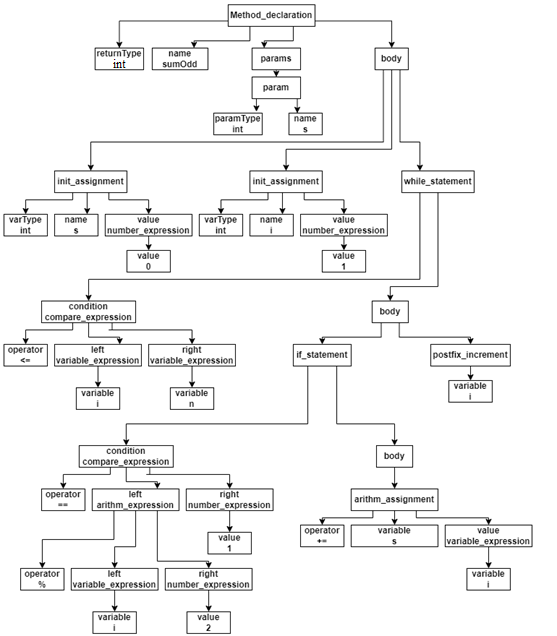
\includegraphics [scale=1] {my_folder/images/my/2}
	\caption{Общая схема статического анализа } 
	\label{fig:2}  
\end{figure}
\section{Граф потока управления} \label{ch1:sec2-abbr2}
Граф потока управления (Control Flow Graph, CFG) — модель программы, представляющая в виде ориентированного графа поток управления в программе. В этой модели сохраняются только инструкции программы, а также информация о возможной передаче управления между инструкциями.
Каждый узел (вершина) графа соответствует базовому блоку - прямолинейному участку кода, не содержащего в себе ни операций передачи управления, ни точек, на которое управление передается из других частей программы. Имеется лишь 2 исключения: точка, на которую выполняется переход, является первой инструкцией в базовом блоке, и базовый блок завершается инструкцией перехода. Направленные дуги используются в графе для представления инструкций перехода. Достижимость — одно из свойств графа, используемое при оптимизациях. Если блок или подграф не имеют путей до них от входного блока, то данная часть графа является недостижимой (мертвый код) при любых вариантах исполнения, и по этой причине он может быть удален из программы. Если же из данного подграфа нет путей до выходного блока, то значит этот подграф содержит бесконечный цикл.
Граф потока управления используется для:
\begin{itemize}
\item Генерации кода 
\item Оптимизации программ 
\item Обнаружения ошибок в программе 
\item И т. п.
\end{itemize}
\begin{figure}[ht!] 
	\center
	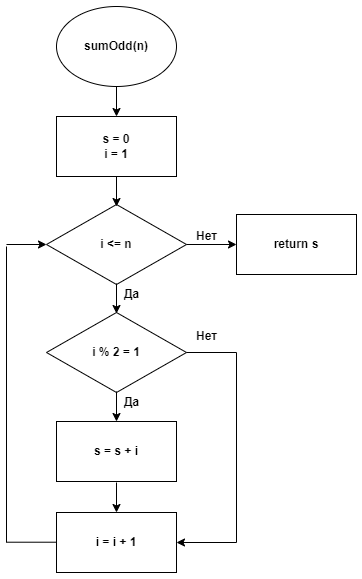
\includegraphics [scale=1] {my_folder/images/my/3}
	\caption{Общая схема статического анализа } 
	\label{fig:3}  
\end{figure}
\section{Граф зависимости по данным} \label{ch1:sec2-abbr3}
Граф зависимостей по данным (Data Dependency Graph, DDG) — модель программы, представляющая в виде направленных дуг зависимости по данным между узлами-инструкциями. Дуга связывает два узла тогда и только тогда, когда между соответствующими инструкциями есть зависимость по данным. Зависимость по данным может иметь один из трех типов: "запись-чтение", "чтение-запись", "запись-запись".
DDG используется при решении задач оптимизации, а также задач автоматизации распараллеливания выполнения. Особенностями данной модели являются относительно небольшое количество типов узлов и связей между ними, простота доступа и навигации.
\begin{figure}[ht!] 
	\center
	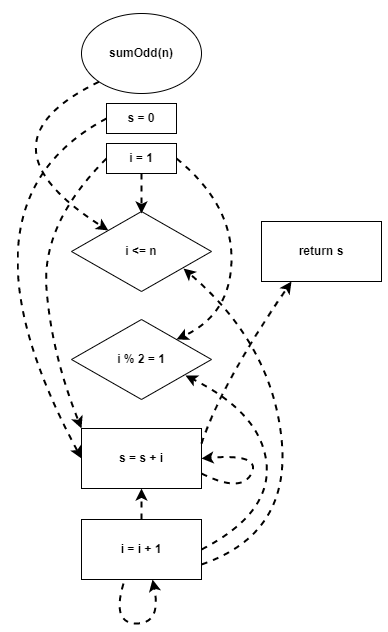
\includegraphics [scale=1] {my_folder/images/my/4}
	\caption{Общая схема статического анализа } 
	\label{fig:4}  
\end{figure}
Исходя из всего вышесказанного, можно сделать вывод, что модели на основе CFG и DDG применимы для отдельных аспектов анализа кода, отражая лишь часть имеющихся зависимостей, и не обладают необходимой полнотой для всестороннего анализа исходного кода.
section{Граф зависимости программы} \label{ch1:sec2-abbr4}
Граф зависимостей программы (Program Dependence Graph, PDG) – это объединенный граф потока данных и графа потока управления. Вершины PDG – это инструкции программы, а ребра – зависимости между ними. Есть две основных типов ребер: ребра выражающие зависимости по данным и ребра выражающие зависимости по управлению.
Граф зависимостей программы используется для:
\begin{itemize}
\item Оптимизации
\item Генерации кода
\item Анализа программ
\item Верификации
\item И т. п.
\end{itemize}	
\begin{figure}[ht!] 
	\center
	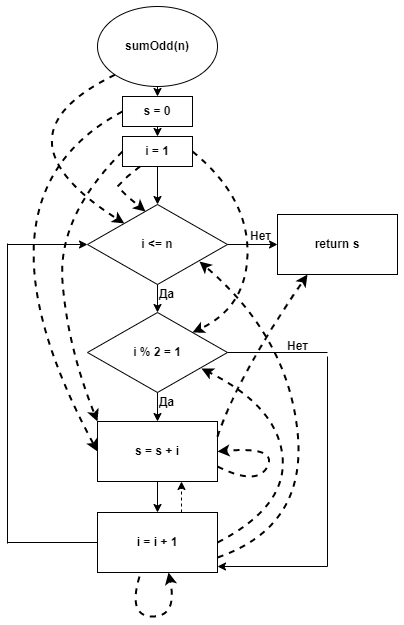
\includegraphics [scale=1] {my_folder/images/my/5}
	\caption{Общая схема статического анализа } 
	\label{fig:5}  
\end{figure}
\section{Абстрактный семантический граф} \label{ch1:sec2-abbr5}
Абстрактный семантический граф (Abstract Semantic Graph, ASG) является расширением AST. ASG по сравнению с AST дополнен различными семантическим дугами, отображающими соответствующие семантические свойства программы и упрощающими навигацию по исходному коду. Данная модель обладает необходимой полнотой для всестороннего анализа исходного кода программы. Для ряда методов статического анализа целесообразно применение упрощенных видов ASG. рассматриваемых как отдельные модели. Подобные модели концентрируются на определенных семантических аспектах, за счет чего размерность и сложность моделей сокращаются.
\begin{figure}[ht!] 
	\center
	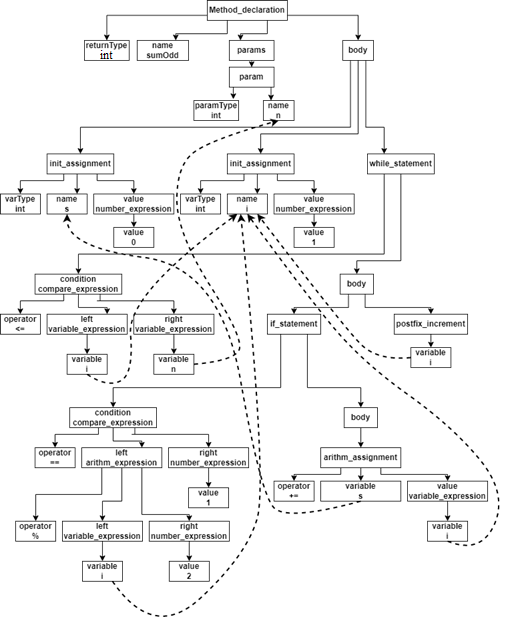
\includegraphics [scale=1] {my_folder/images/my/6}
	\caption{Общая схема статического анализа } 
	\label{fig:6}  
\end{figure}
\section{Представление на основе однократного статического присваивания} \label{ch1:sec2-abbr6}
Представление на основе однократного статического присваивания (static single assignment, SSA) – это представление исходного кода программы, в котором:
\begin{itemize}
\item Каждой локальной переменной значение присваивается только один раз.
\item Вводится версионирование для локальных переменных, которые в исходном коде имеют неоднократные присваивания.
\item Для локальных переменных вводятся Фи-функции на выходе условных конструкций, объединяющие несколько ветвей программы и определяющие их окончательное значение
\item Циклы заменяются инструкциями ветвления и безусловных переходов
\end{itemize}
Данное представление может быть изображено в CFG-форме.
\begin{figure}[ht!] 
	\center
	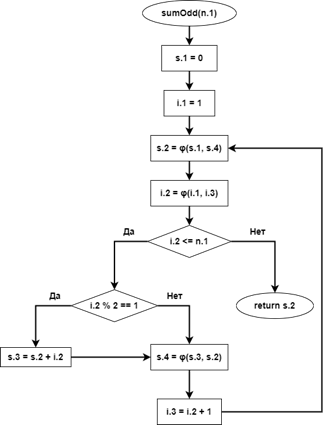
\includegraphics [scale=1] {my_folder/images/my/7}
	\caption{Общая схема статического анализа } 
	\label{fig:7}  
\end{figure}
\section{Выводы по главе} \label{ch1:sec3}
В данной главе были изучены методики исправления ошибок в программном коде и проведен анализ предметной области. Для каждой модели приведен теоретический обзор и представлен один из вариантов визуализации. Модельное представление программы призвано упростить и формализовать разработку алгоритмов статического анализа. При этом выбранное модельное представление должно обладать определенными свойствами, обеспечивающими эффективность и наглядность алгоритмов статического анализа.

\newpage





% не рекомендуется использовать отдельную section <<введение>> после лета 2020 года
%\section{Введение. Сложносоставное название первого параграфа первой главы для~демонстрации переноса слов в содержании} \label{ch1:intro}


%\section{Название параграфа} \label{ch1:sec1}
%
%
%\subsection{Название первого подпараграфа первого параграфа первой главы для~демонстрации переноса слов в содержании} % ~ нужен, чтобы избавиться от висячего предлога (союза) в конце строки
%
%Содержание первого подпараграфа первого параграфа первой главы.
%
%
%
%Одиночные формулы оформляют в окружении \texttt{equation}, например, как указано в следующей одиночной нумерованной формуле:
%%
%%
%\begin{equation}% лучше не оставлять пропущенную строку (\par) перед окружениями для избежания лишних отсупов в pdf
%\label{eq:Pi-ch1} % eq - equations, далее название, ch поставлено для избежания дублирования
%\pi \approx 3,141.
%\end{equation}
%%
%%
%\begin{figure}[ht!] 
%	\center
%	\includegraphics [scale=0.27] {my_folder/images//spbpu_hydrotower}
%	\caption{Вид на гидробашню СПбПУ \cite{spbpu-gallery}} 
%	\label{fig:spbpu_hydrotower}  
%\end{figure}
%%
%%
%%\begin{table} [htbp]% Пример оформления таблицы
%%	\centering\small
%%	\caption{Представление данных для сквозного примера по ВКР \cite{Peskov2004}}%
%%	\label{tab:ToyCompare}		
%%		\begin{tabular}{|l|l|l|l|l|l|}
%%			\hline
%%			$G$&$m_1$&$m_2$&$m_3$&$m_4$&$K$\\
%%			\hline
%%			$g_1$&0&1&1&0&1\\ \hline
%%			$g_2$&1&2&0&1&1\\ \hline
%%			$g_3$&0&1&0&1&1\\ \hline
%%			$g_4$&1&2&1&0&2\\ \hline
%%			$g_5$&1&1&0&1&2\\ \hline
%%			$g_6$&1&1&1&2&2\\ \hline		
%%		\end{tabular}	
%%	\normalsize% возвращаем шрифт к нормальному
%%\end{table}
%
%
%% \firef{} от figure reference
%% \taref{} от table reference
%% \eqref{} от equation reference
%
%На \firef{fig:spbpu_hydrotower} изображена гидробашня СПбПУ, а в \taref{tab:ToyCompare} приведены данные, на примере которых коротко и наглядно будет изложена суть ВКР.
%
%
%\section{Название параграфа} \label{ch1:sec2} 
%
%
%
%Формулы могут быть размещены в несколько строк. Чтобы выставить номер формулы напротив средней строки, используйте окружение \verb|multlined| из пакета \verb|mathtools| следующим образом \cite{Ganter1999}:
%%
%\begin{equation} 
%\label{eq:fConcept-order-ch1}
%\begin{multlined}
%(A_1,B_1)\leq (A_2,B_2)\; \Leftrightarrow \\  \Leftrightarrow\; A_1\subseteq A_2\; \Leftrightarrow \\ \Leftrightarrow\; B_2\subseteq B_1. 
%\end{multlined}
%\end{equation}
%
%
%Используя команду \verb|\labelcref| из пакета \verb|cleveref|, допустимо следующим образом оформлять ссылку на несколько формул:
%(\labelcref{eq:Pi-ch1,eq:fConcept-order-ch1}).
%%
%%
%\input{my_folder/tex/fig-spbpu-whitehall-three-in-one} % пример подключения 3х иллюстрации в одном рисунке
%
%Пример ссылок \cite{Article,Book,Booklet,Conference,Inbook,Incollection,Manual,Mastersthesis,Misc,Phdthesis,Proceedings,Techreport,Unpublished,badiou:briefings}, а также ссылок с указанием страниц, на котором отображены номера страниц  \cite[с.~96]{Naidenova2017} или в виде мультицитаты на несколько источников \cites[с.~96]{Naidenova2017}[с.~46]{Ganter1999}. Часть библиографических записей носит иллюстративный характер и не имеет отношения к реальной литературе. 
%
%
%
%%\FloatBarrier % заставить рисунки и другие подвижные (float) элементы остановиться
%
%\section{Выводы} \label{ch1:conclusion}
%
%Текст выводов по главе \thechapter.
%
%Кроме названия параграфа <<выводы>> можно использовать (единообразно по всем главам) следующие подходы к именованию последних разделов с результатами по главам:
%\begin{itemize}
%	\item <<выводы по главе N>>, где N --- номер соответствующей главы;
%	\item <<резюме>>;
%	\item <<резюме по главе N>>, где N --- номер соответствующей главы.
%\end{itemize}
%
%Параграф с изложением выводов по главе \textit{является обязательным}.
%
%%% Вспомогательные команды - Additional commands
%%
%%\newpage % принудительное начало с новой страницы, использовать только в конце раздела
%%\clearpage % осуществляется пакетом <<placeins>> в пределах секций
%%\newpage\leavevmode\thispagestyle{empty}\newpage % 100 % начало новой страницы	         	 % Глава 1
\ContinueChapterBegin % размещать главы <<подряд>> 
\chapter{Обзор существующих решений} \label{ch2}
В данной главе будут рассмотрены существующие средства визуализации, определены их плюсы и минусы и указан краткий обзор.
\section{Анализ существующих средств визуализации моделей программ} \label{ch2:sec1}
Существует множество вариантов архитектуры визуализатора. Это может быть как десктопное приложение, как мобильное, как клиент-серверное. Для анализа были выбраны визуализаторы, находящиеся в свободном доступе и максимально приближенные к желаемому результату.
\subsection{VisualDFA} \label{ch2:subsec-title-abbr}
VisualDFA – это сложный образовательный инструмент для визуализации анализа потоков данных с использованием Java/Jimple, который позволяет:
\begin{itemize}
\item Запускать 4 встроенных анализа: сворачивание констант (Constant Folding), биты констант (Constant Bits), достигающие определения (Reaching Definitions) и проверка на заражённость (Taint Analysis)
\item Вводить Java-код, либо подключать его из файла
\item Визуализировать код с помощью CFG
\item Выполнять код пошагово, либо продолжить до следующей установленной точки остановки
\item Видеть входные и выходные данные для любого блока или строки кода в любой момент времени
\item Экспорт CFG в PNG-файл или вывод одной командой изображений всех шагов анализа
\item Внедрять и запускать пользовательские анализы без перекомпиляции VisualDFA
\end{itemize}

Этот инструмент строит CFG в интерфейсе своего приложения. Внешний вид получаемого CFG не такой, как хотелось бы его видеть. У каждого блока вверху есть пустая область, за которую блок можно перетаскивать. При этом во время перетаскивания размещение стрелок происходит странным образом. Они пересекают другие блоки и частично остаются на начальных позициях. Так же блоки начала метода, условий и обычных операторов визуально не отличаются. От условий идут стрелки, смотря на которые непонятно, по какой из них переходить в случае, если условие истинно, и по какой в случае, если ложно. Создаются временные переменные там, где их нет в коде. Почему-то сами условия записываются противоположно тем, которые написаны в коде.

Как итог, VisualDFA можно назвать готовым решением для построения и визуализации CFG, но результат оставляет желать лучшего. На рис. 2.1 изображен результат работы VisualDFA.\\

\begin{figure}[h]
	\center
	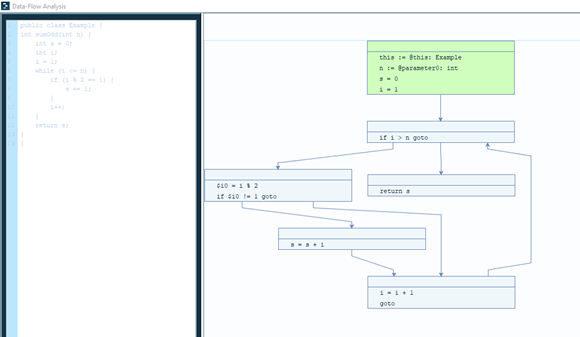
\includegraphics [scale=1] {my_folder/images/my/10}
	\caption{Результат работы VisualDFA}
	\label{fig:10}
\end{figure}

\subsection{VisualControlFlowGraph4J} \label{ch2:subsec-title-abbr}
VisualControlFlowGraph4J – инструмент для построения и визуализации Java-кода в виде CFG, использующий ANTLR и GraphViz.
Инструмент помогает строить CFG, но у него также есть ряд недостатков. Построение CFG нельзя назвать интерактивным. Он требует файла с исходным кодом в папке с ресурсами для того, чтобы строить модель по нему. Граф сохраняется в файловую систему в виде SVG-файла по завершению работы программы. В самом CFG присутствуют обозначения типов данных, что делает граф привязанным к языку программирования. Также наблюдается проблема с тем, что, смотря на стрелки, исходящие из блоков условий, непонятно, по какой из них переходить при истинном или ложном условии. Кроме того, никак не обозначены параметры метода, граф для которого строится.
VisualControlFlowGraph4J можно считать готовым решением для построения и визуализации CFG, но не лишённым своих недостатков. На рис. 2.2 изображен результат работы VisualControlFlowGraph4J.

\begin{figure}[h]
	\center
	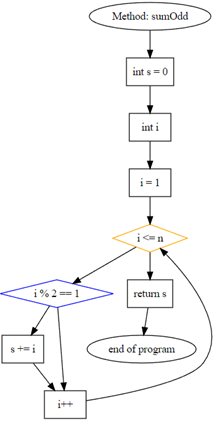
\includegraphics [scale=1.1] {my_folder/images/my/11}
	\caption{Результат работы VisualControlFlowGraph4J}
	\label{fig:11}
\end{figure}

\subsection{ANTLR} \label{ch2:subsec-title-abbr}
ANTLR (Another Tool for Language Recognition) – это мощный генератор парсеров. С его помощью можно сгенерировать парсер для любой заданной грамматики, в том числе для языков программирования. Для генерации парсера нужен файл грамматики, составленный по определённым правилам. Существует множество готовых грамматик для разных языков, в том числе для языка программирования Java. Кроме того, есть возможность вывести дерево парсинга в графическом интерфейсе.
Сам по себе ANTLR не является готовым решением для построения и визуализации AST. Он лишь может сгенерировать код по шаблону (Visitor или Listener) на одном из поддерживаемых языков программирования, который можно дописать для получения желаемого результата. Дерево парсинга, которое получается при использовании ANTLR, содержит в себе все символы исходного текста. Чтобы из этого построить AST, необходимо убрать множество лишних элементов. На рис. 2.3 изображен графический интерфейс ANTLR.

\begin{figure}[h]
	\center
	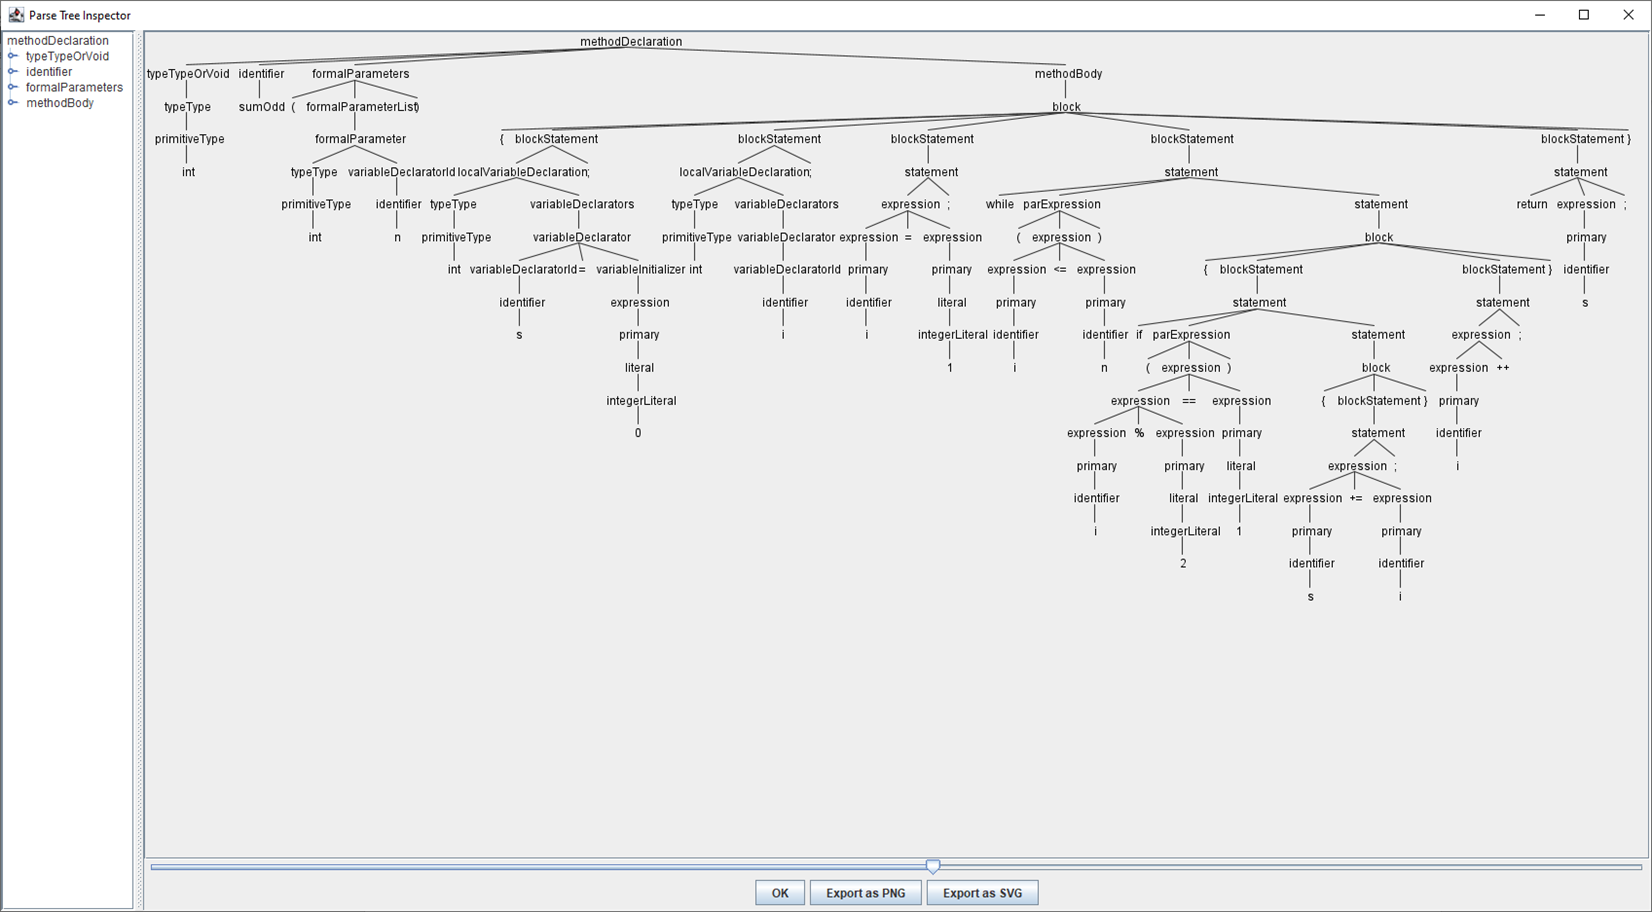
\includegraphics [scale=0.38] {my_folder/images/my/8}
	\caption{Графический интерфейс ANTLR}
	\label{fig:8}
\end{figure}

\subsection{AST Explorer} \label{ch2:subsec-title-abbr}
AST Explorer – это инструмент для парсинга кода на разных языках, в том числе Java, который использует Node.js в качестве сервера и содержит ссылки на каждый пакет в репозитории npm, используемый в качестве парсера для того или иного языка.
Из способов визуализации поддерживается только вывод в виде интерактивного иерархического текста, либо в виде кода JSON. И строится в результате не AST, а дерево парсинга, которое тоже содержит множество ненужных для построения AST узлов.
Таким образом, его тоже нельзя назвать готовым решением для построения и визуализации AST для кода на языке Java. На рис. 2.4 изображен результат работы AST Explorer.
\newpage

\begin{figure}[h]
	\center
	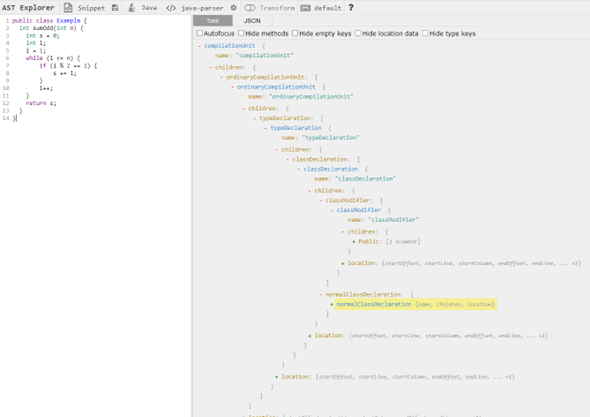
\includegraphics [scale=1] {my_folder/images/my/9}
	\caption{Результат работы AST Explorer}
	\label{fig:9}
\end{figure}

\section{Выводы по главе} \label{ch2:sec2}
В данной главе проведен обзор и анализ существующих средств визуализации моделей программ. Были найдены лишь решения для AST и CFG, для визуализации остальных моделей программ не было найдено ни одного достойного решения. Также хочется отметить, что не существует ни одного сервиса, способного интерактивно визуализировать несколько разных моделей программ. На основе результата обзора можно сделать вывод о том, что тема выпускной квалификационной работы является актуальной.
\newpage	         	 % Глава 2
\chapter{Постановка задачи и разработка требований к системе} \label{ch3}
В данной главе производится постановка задачи и разработка требований к сервису интерактивной визуализации моделей программ.
\section{Постановка задачи} \label{ch3:sec1}
Исходя из анализа существующих решений можно сделать вывод, что не существует интерактивного визуализатора, отображающего все заявленные модели программ, поэтому необходимо разработать систему для интерактивной визуализации моделей кода на языке Java, а именно:
\begin{itemize}
\item AST
\item CFG
\item DDG
\item PDG
\item ASG
\item SSA
\end{itemize}
Для выполнения этой задачи требуется:
\begin{itemize}
\item Разработать требования к системе
\item Спроектировать архитектуру сервиса
\item Проанализировать и выбрать средства решения
\item Разработать сервис в соответствии с установленными требованиями
\item Протестировать и отладить разработанный сервис
\end{itemize}
\section{Разработка требований к системе} \label{ch3:sec2}
Необходимо разработать сервис, позволяющий получать код метода на языке Java от пользователя и строить по этому коду визуализацию выбранной модели.
Общие требования: 
\begin{itemize}
\item Сервис должен быть интерактивным
\end{itemize}
Любое изменение кода должно приводить к изменению модели без дополнительных действий со стороны пользователя. Если введённый код некорректен, сервис должен сообщить пользователю об этом.
\begin{itemize}
\item Сервис должен работать на компьютерах, смартфонах и планшетах
\end{itemize}
Должна быть возможность воспользоваться сервисом с любых устройств, на которых есть браузер.
\begin{itemize}
\item Сервис должен позволять строить все обозначенные модели через единый интерфейс
\end{itemize}
Это AST, CFG, DDG, PDG, ASG и SSA. У пользователя должна быть возможность переключаться между моделями.
\begin{itemize}
\item Удобная навигация по большим моделям
\end{itemize}
Должна быть возможность изменения масштаба изображения модели, а также возможность его перемещения внутри области просмотра.
\begin{itemize}
\item Элементы графов должны размещаться детерминировано
\end{itemize}
Для одного и того же кода необходимо всегда получать одинаковую визуализацию всех моделей.
Уточняющие требования по AST:
\begin{itemize}
\item В дереве должны присутствовать только семантически значимые узлы
\item Должна быть возможность сворачивать и разворачивать поддеревья
\end{itemize}
Уточняющие требования по CFG:
\begin{itemize}
\item Необходимо использовать стандартные формы для обозначения узлов
\end{itemize}
Эллипс для обозначения начала или конца, прямоугольник для обычных операторов, ромб для узлов принятия решений.
\begin{itemize}
\item Метки на рёбрах из узлов принятия решений
\end{itemize}
Рёбра, выходящие из узлов принятия решений, должны иметь обозначения, дающие понять пользователю, по какому ребру переходить в случае, если условие истинно, а по какому в случае, если ложно.
\begin{itemize}
\item Граф не должен быть привязан к языку программирования
\end{itemize}
Нужно убрать типы данных из названий узлов, а также объявления переменных без инициализации. Конструкции if, for и while должны быть отображены как условия с необходимыми стрелками. Инструкции break и continue не должны появляться как самостоятельные узлы, а должны только влиять на расположение стрелок.
\section{Выводы по главе} \label{ch3:sec3}
В этой главе была поставлена задача, которую необходимо решить в рамках выпускной квалификационной работы и определены требования для реализации сервиса интерактивной визуализации моделей программ.
\newpage




% не рекомендуется использовать отдельную section <<введение>> после лета 2020 года
%\section{Введение} \label{ch3:intro}

%Хорошим стилем является наличие введения к главе. Во введении может быть описана цель написания главы, а также приведена краткая структура главы. 
%	
%\section{Название параграфа} \label{ch3:sec1}
%
%\section{Название параграфа} \label{ch3:sec2}
%
%%\FloatBarrier % заставить рисунки и другие подвижные (float) элементы остановиться
%
%
%\section{Выводы} \label{ch3:conclusion}
%
%Текст выводов по главе \thechapter.
%
%
%%% Вспомогательные команды - Additional commands
%%
%%\newpage % принудительное начало с новой страницы, использовать только в конце раздела
%%\clearpage % осуществляется пакетом <<placeins>> в пределах секций
%%\newpage\leavevmode\thispagestyle{empty}\newpage % 100 % начало новой страницы           	 % Глава 3
\chapter{Проектирование архитектуры и выбор средств решения} \label{ch4}
Для реализации интерактивного визуализатора моделей программ необходимо решить следующие подзадачи:
\begin{itemize}
\item Получение из исходного кода метода на языке Java абстрактного синтаксического дерева
\item Обеспечение отрисовки деревьев и графов в браузере
\item Преобразование структуры AST в данные для отрисовки AST, CFG, DDG, PDG, ASG и SSA
\item Создание интерфейса для взаимодействия с программой
\end{itemize}
\begin{figure}[ht!] 
	\center
	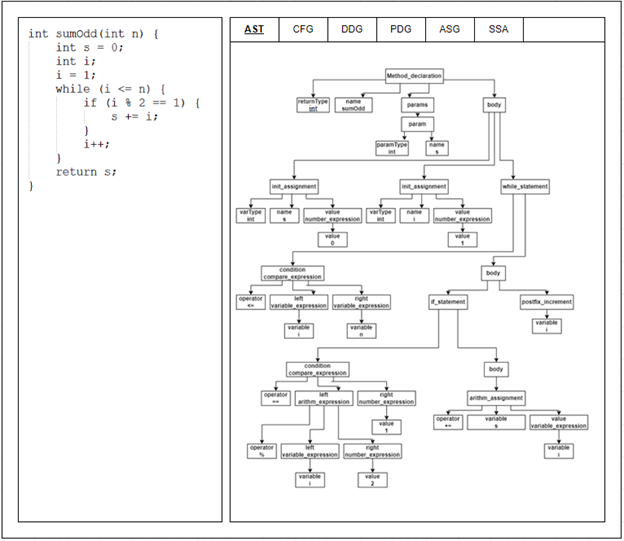
\includegraphics [scale=0.27] {my_folder/images/my/12}
	\caption{Схематичное представление интерфейса визуализатора} 
	\label{fig:12}  
\end{figure}
\section{Парсинг кода} \label{ch4:sec1}
Для парсинга кода можно использовать существующие парсеры, либо же разработать свой.
\begin{itemize}
\item Существующие парсеры
\end{itemize}
Плюсы: не нужно тратить время на разработку, наверняка работает как ожидается.
Минусы: обычно работает не так, как хотелось бы, очень сложно изменить что-то, обычно решение громоздкое, нужно тратить время, чтобы найти готовое решение, и разобраться в нём.
\begin{itemize}
\item Разработка своего парсера
\end{itemize}
Плюсы: можно разработать именно так, как нужно, достаточно компактно, без лишнего нагромождения функционала.
Минусы: Процесс слишком долгий и трудоемкий.
Из готовых решений хочется выделить ANTLR и JavaParser.
\subsection{ANTLR} \label{ch2:subsec-title-abbr}
%\section{ANTLR} \label{ch4:sec1-abbr}
ANTLR. Универсальный парсер, в котором есть готовые грамматики почти под любой язык, в том числе Java. Результатом работы является parse tree. Если мы хотим избавиться от лишней для AST информации, то требуется дописать большое количество программного кода. Также у данного парсера нет сериализации в JSON.
%\section{JavaParser} \label{ch4:sec1-abbr}
\subsection{JavaParser} \label{ch2:subsec-title-abbr}
JavaParser заточен под Java и выдаёт структуру только из семантически значимых элементов, что очень удобно. Реализована встроенная сериализация в JSON, но выдаётся куча вспомогательной информации, AST из такого строить неудобно, поэтому требуется писать упрощённый сериализатор.
Исходя из всех вышеуказанных плюсов и минусов было принято решение воспользоваться JavaParser. Он не работает в браузере, поэтому нужен сервер. Таким образом, нужно использовать клиент-серверную архитектуру. Будет приложение в браузере, которое отправляет запросы на сервер, чтобы получить результат работы JavaParser.
\section{Выбор фреймворка для сервера} \label{ch4:sec2}
Для Java существует множество различных http-фреймворков. Самый популярный из них Spring, так же существует очень простой фреймворк Spark.
\begin{itemize}
\item Spring - очень мощный и большой фреймворк, популярный и сложный. Избыточный для поставленных задач
\item Spark - простой и минималистичный, вполне достаточный для наших задач
\end{itemize}
\section{Выбор способа визуализации} \label{ch4:sec3}
Для выбора способа визуализации нужно определиться, использовать готовую библиотеку или писать свое решение.
Существует множество библиотек для отрисовки графов, требуется выбрать наилучшую для реализации поставленных задач.
\begin{itemize}
\item Dracula Graph Library – размещает узлы хаотично, а так же сам вид визуализации не подходит для требуемого сервиса.
\end{itemize}
\begin{figure}[ht!] 
	\center
	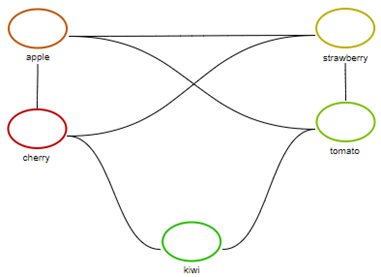
\includegraphics [scale=0.27] {my_folder/images/my/13}
	\caption{Пример результата, выдаваемого библиотекой Dracula Graph Library} 
	\label{fig:13}  
\end{figure}
\begin{itemize}
\item Vis.js – размещает узлы не так, как хотелось бы (по принципу “упругого” физического движка), а так же сам вид визуализации не подходит для требуемого сервиса.
\end{itemize}
\begin{figure}[ht!] 
	\center
	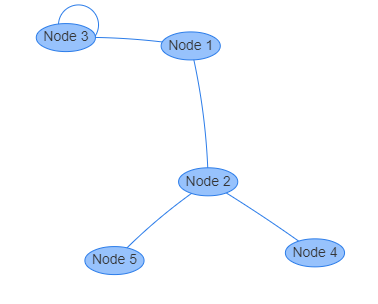
\includegraphics [scale=0.27] {my_folder/images/my/14}
	\caption{Пример результата, выдаваемого библиотекой Vis.js} 
	\label{fig:14}  
\end{figure}
\begin{itemize}
\item Cytoscape.js – так же размещает узлы хаотично.
\end{itemize}
\begin{figure}[ht!] 
	\center
	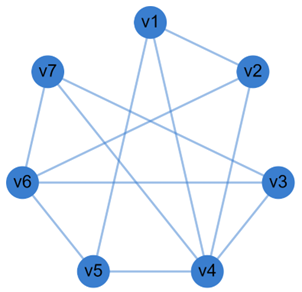
\includegraphics [scale=0.27] {my_folder/images/my/15}
	\caption{Пример результата, выдаваемого библиотекой Cytoscape.js} 
	\label{fig:15}  
\end{figure}
\begin{itemize}
\item JavaScript InfoVis Toolkit (JIT) - неплохо рисует деревья, но плохо рисует графы. Как и предыдущие библиотеки хаотично размещает узлы и ребра и не подходит по виду визуализации.
\end{itemize}
\begin{figure}[ht!] 
	\center
	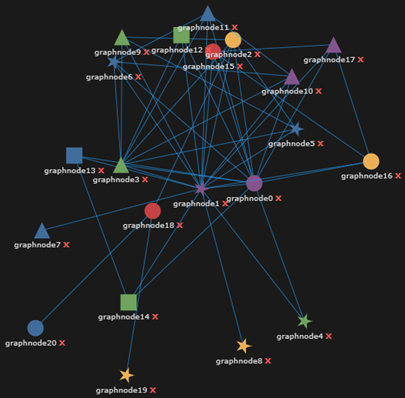
\includegraphics [scale=0.27] {my_folder/images/my/16}
	\caption{Пример результата, выдаваемого библиотекой JIT} 
	\label{fig:16}  
\end{figure}
\begin{itemize}
\item D3.js – позволяет визуализировать очень много всего, но не то, что нужно для нашего сервиса. Тоже имеет “упругое” размещение и не обладает нужным видом.
\end{itemize}
\begin{figure}[ht!] 
	\center
	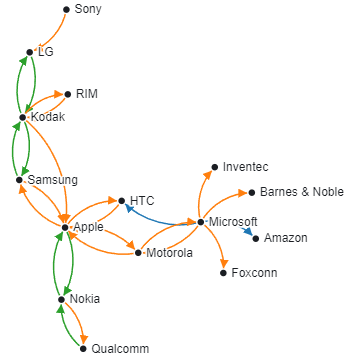
\includegraphics [scale=0.27] {my_folder/images/my/17}
	\caption{Пример результата, выдаваемого библиотекой D3.js} 
	\label{fig:17}  
\end{figure}
\begin{itemize}
\item Sigma.js - требует задания координат в XML и не обладает нужным видом.
\end{itemize}
\begin{figure}[ht!] 
	\center
	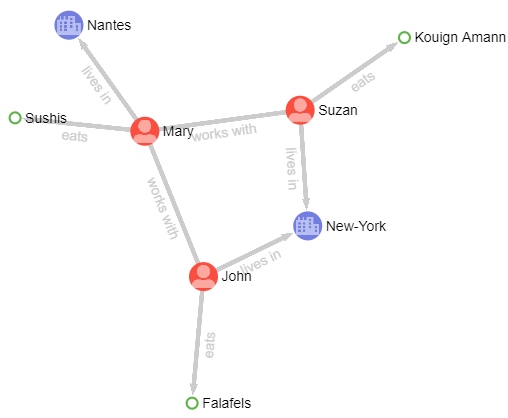
\includegraphics [scale=0.27] {my_folder/images/my/18}
	\caption{Пример результата, выдаваемого библиотекой Sigma.js} 
	\label{fig:18}  
\end{figure}
\begin{itemize}
\item Graphviz - был скомпилирован для Javascript с использованием Emscripten в формат WebAssembly. Существует в виде плагина к библиотеке D3.js. Умеет визуализировать графы с настраиваемым размещением и видом узлов, а также, отображает графы, описанные на языке DOT – универсальном языке описания графов.
Так же стоит рассмотреть вариант создания собственной визуализации.
\item Плюсы: достаточно компактное решение, которое делает именно то, что нужно
\item Минусы: сложная логика размещения и очень затратное по времени решение
\end{itemize}
Исходя из всего вышесказанного выбор пал на d3-graphviz, так как это наиболее подходящий вариант для нашего сервиса.
\section{Интерфейс взаимодействия с программой} \label{ch4:sec4}
Требуется создать интерфейс для взаимодействия с программой, для этого нужно определиться использовать или не использовать фреймворк.
Фреймворк – это инструмент для построения приложений. Обычно фреймворки определяют структуру приложения. Кроме того, они содержат множество уже готовых модулей, упрощающих разработку. В случае с JavaScript фреймворки помогают писать декларативный код, а не императивный. При использовании фреймворка обычно используются сборщики проекта. Как правило, настройка сборщика по умолчанию уже включает в себя компилятор babel, а также минификацию HTML, CSS и JavaScript кода. Минификация уменьшает размер и количество подключаемых файлов, что положительно сказывается на времени загрузки страниц. Babel позволяет писать код на новых версиях JavaScript, и он будет преобразован в JavaScript более старых версий, что увеличивает поддержку браузерами. Кроме этого, фреймворки добавляют плагины к babel, что позволяет использовать синтаксические конструкции, которых нет в чистом JavaScript. Кроме того, фреймворки позволяют запускать сервер для разработки, благодаря которому происходит отслеживание изменений в коде в режиме реального времени, и все изменения видны в браузере сразу без перезагрузки страницы.
Таким образом, можно сделать вывод, что фреймворки ускоряют и упрощают процесс разработки. Минус фреймворка заключается в том, что его код также включается в сборку, из-за чего JavaScript кода, который нужно загрузить в браузер, становится больше, что в некоторой степени замедляет первоначальную загрузку страницы. Было принято решение использовать фреймворк.
\section{Выбор фреймворка} \label{ch4:sec5}
1.	React
\begin{itemize}
\item Плюсы: большое сообщество, множество дополнительных библиотек, самый популярный на сегодняшний день, использует Virtual DOM (что улучшает производительность)
\item Минусы: громоздкий синтаксис, относительная сложность освоения, плохо структурированная документация, нестрогая структура приложения
\end{itemize}
2.	Angular
\begin{itemize}
\item Плюсы: огромный, мощный фреймворк, встроенная строгая типизация, множество встроенных возможностей, строгая структура приложения, хорошая документация
\item Минусы: сложно освоить, не использует Virtual DOM, большой размер, излишний для небольших проектов
\end{itemize}
3.	Vue.js
\begin{itemize}
\item Плюсы: очень простой и лёгкий в освоении, использует Virtual DOM (что улучшает производительность), хорошая документация, достаточно популярный
\item Минусы: не очень развитое сообщество, нестрогая структура приложения
\end{itemize}
4.	Svelte
\begin{itemize}
\item Плюсы: минимальный размер выходного приложения, простой в освоении, максимально производительный код на выходе
\item Минусы: очень молодой, непопулярный проект, маленькое сообщество
\end{itemize}
Проанализировав плюсы и минусы различных фреймворков, было принято решение, что для создания визуализатора самым подходящим будет Vue.js. Для обращений к серверу решено использовать библиотеку axios, как самое популярное решение для подобных задач, а в качестве готовых стилей для оформления интерфейса выбран CSS-фреймворк bulma.
\section{Выводы по главе} \label{ch4:sec6}
В данной главе описана архитектура и были выбраны средства решения. При создании сервиса будет использована клиент-серверная архитектура с использованием фреймворка Spark на стороне сервера и фреймворка Vue.js на стороне клиента. В качестве дополнительных инструментов будут использоваться JavaParser на стороне сервера для парсинга кода, Gson для сериализации в JSON. На стороне клиента будут использоваться axios для сетевых запросов, bulma для оформления интерфейса, d3 и d3-graphviz для отрисовки деревьев и графов.
\begin{figure}[ht!] 
	\center
	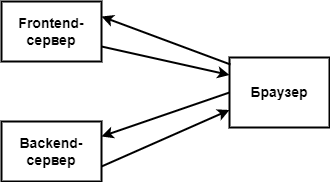
\includegraphics [scale=0.27] {my_folder/images/my/19}
	\caption{Схема работы сервиса} 
	\label{fig:19}  
\end{figure}
Когда пользователь открывает сервис в браузере, он обращается к Frontend серверу, откуда получает статические файлы HTML, CSS, JavaScript и другие, далее браузер строит по этим файлам страницу. Когда пользователь вводит код в интерфейсе, происходит запрос к Backend-серверу (его адрес прописывается в JavaScript от Frontend-сервера). Ответ от сервера обрабатывается браузером при помощи JavaScript-кода с Frontend-сервера.
\newpage














% не рекомендуется использовать отдельную section <<введение>> после лета 2020 года
%\section{Введение} \label{ch4:intro}

%Хорошим стилем является наличие введения к главе. Во введении может быть описана цель написания главы, а также приведена краткая структура главы. 
%	
%\section{Название параграфа} \label{ch4:sec1}
%
%\section{Название параграфа} \label{ch4:sec2}
%
%Пример ссылки на литературу \cite{avtonomova:fya,Peskov2004-ru,Kotelnikov2004-ru,Kotelnikov2004}.
%
%%\FloatBarrier % заставить рисунки и другие подвижные (float) элементы остановиться
%
%\section{Выводы} \label{ch4:conclusion}
%
%Текст выводов по главе \thechapter.
%
%%% Вспомогательные команды - Additional commands
%%
%%\newpage % принудительное начало с новой страницы, использовать только в конце раздела
%%\clearpage % осуществляется пакетом <<placeins>> в пределах секций
%%\newpage\leavevmode\thispagestyle{empty}\newpage % 100 % начало новой страницы           	 % Глава 4
\chapter{Разработка сервиса интерактивного визуализатора моделей программ} \label{ch5}
В данной главе описывается разработка сервиса интерактивного визуализатора моделей программ. Для разработки сервера выбран язык программирования Java, для разработки клиента – JavaScript.
\section{Разработка сервера} \label{ch5:sec1}
Главная задача сервера – отвечать по протоколу HTTP на запросы от клиента. В нашем случае будет одна основная точка доступа, на вход которой подаётся исходный код на языке Java, а в качестве ответа ожидается JSON, в котором будет содержаться структура AST в двух видах – в облегчённом (для рисования) и в расширенном (с указанием связей с исходным кодом).
Для реализации этой логики были созданы следующие классы:
\begin{itemize}
\item Main – содержит главный метод приложения. В нём описаны точки доступа и их поведение. В том числе точка доступа для обеспечения корректной работы кросс-доменных запросов (настройка CORS), и главная точка доступа приложения для преобразования кода в AST.
\item JsonPrinter – класс для преобразования объектной структуры AST в облегчённую версию JSON. Этот класс был удалён из библиотеки JavaParser. Разработчики изменили способ сериализации, оставив только возможность генерации JSON расширенной версии AST. Расширенная версия включает в себя дополнительную информацию, в том числе номера начальных и конечных строк и столбцов для каждого узла, номера токенов, а также пустые ключи для всех синтаксически допустимых элементов, не встречающихся в коде (например, аннотаций для методов и переменных, бросаемые исключения и прочее). Поскольку облегченная версия всё-таки оказалась нужна, пришлось добавить этот класс.
\item Response – структурный класс, содержащий поля status и data. Создан для стандартизации вида ответов сервера (status может иметь значение “success” или “error”, data – любые данные). Задаёт структуру ответа сервера при сериализации в JSON.
\item AstResponse – структурный класс, содержащий поля simple и extended (для облегчённой и расширенной версии AST, соответственно). Используется в основной точке доступа как значение поля data в объекте Response при ответе.
\end{itemize}
\section{Разработка клиента} \label{ch5:sec2}
Клиент включает в себя практически всю логику приложения. Ниже описана разработка для каждой модели.
\subsection{Построение AST} \label{ch2:subsec-title-abbr}
Для построения AST нужно использовать облегчённую версию структуры, полученной от сервера. Задача сводится к преобразованию этой иерархической структуры в код графа на языке DOT. Для этого необходимо описать каждый узел дерева и каждое ребро, соединяющее узлы. Кроме того, необходимо реализовать функционал сворачивания и разворачивания поддеревьев по клику на узел.

Для получения массива узлов и массива рёбер нужно выполнить рекурсивный обход AST-структуры. В зависимости от типа полей требуется выполнять разные действия. Если тип поля – массив, нужно добавить узел с именем поля, на каждом элементе рекурсивно вызвать обход, добавляя рёбра от только что созданного узла к корневым узлам поддеревьев, созданных в каждом внутреннем обходе. Если тип поля – объект, нужно отделить поле с типом узла от остальных (значение этого поля установится как имя узла). Для всех остальных полей нужно запустить рекурсивный обход, добавляя необходимые рёбра. Если тип поля – примитив, то и название, и значение поля будут установлены в названии узла.

Для реализации функционала сворачивания и разворачивания поддеревьев необходимо каким-то образом обозначить связи между отображаемыми узлами дерева, чтобы можно было определять, является ли тот или иной узел дерева потомком другого. Это можно делать по данным из массива рёбер, но такой алгоритм будет неэффективным. Поэтому было принято решение сделать у каждого узла ссылку на родительский узел. Пройдя циклом по цепочке родительских элементов, можно понять, является ли какой-то узел потомком другого. Далее создадим множество из индексов узлов для хранения информации о корнях свёрнутых пользователем поддеревьев. При клике на узел нужно получить индекс того узла, по которому произошёл клик. Если такой индекс есть во множестве, тогда его нужно удалить из множества, а если нет, то добавить. После этого пройти по всем узлам и рёбрам, и пометить скрытыми те узлы, которые являются потомками хотя бы одного из узлов во множестве, и те рёбра, которые ведут на такие узлы (которые помечаем скрытыми).

Для создания кода графа на языке DOT достаточно создать по одной строке для каждого не скрытого узла и для каждого не скрытого ребра, а затем объединить эти строки в соответствии с синтаксисом языка DOT.

\subsection{Построение CFG} \label{ch2:subsec-title-abbr}
Для построения CFG нужно использовать расширенную версию структуры, полученной от сервера. Задача также сводится к преобразованию этих данных в код графа на языке DOT.

Входные данные – AST-дерево, описывающее код. Нужно каким-то образом определять, какие элементы будут являться узлами графа, какой текст будет в них содержаться, и какие пары из них будут соединены ориентированными рёбрами. Кроме того, узлы должны иметь разные формы, в зависимости от их типа, и некоторые рёбра должны иметь подписи “да” и “нет”, в случае если они выходят из узла-условия.

AST содержит множество типов узлов. Для удобства обхода этой структуры было решено воспользоваться адаптацией ООП-паттерна «Посетитель» (Visitor). В зависимости от типа узла, будут выполняться различные действия. В частности, необходимо описать различные действия на узлах объявления метода, объявления переменных, блоков кода, циклов while, циклов for, ветвлений if, инструкций return, break и continue. Для всех остальных типов узлов, вложенных непосредственно в перечисленные, будет создаваться отдельный узел графа, текстом для которого будет код, по которому был построен данный узел AST дерева.

Была определена процедура добавления узла. Кроме того, что она создаёт узел и добавляет его в массив узлов, она ещё ставит все необходимые рёбра в этот узел. Это реализовано за счёт создания глобального списка частично определённых рёбер (для удобства обозначим аббревиатурой ЧОР, у которых указаны начало и тип, но не указан конец). Эта процедура извлекает все значения из этого списка, добавляет в каждое ЧОР конечным узлом себя, и добавляет каждое полученное ребро в массив рёбер. Также добавляет в список ЧОР единственным элементом ЧОР, в котором началом указан новый узел, а типом – ребро без подписи. Дальнейшие инструкции (после процедуры) могут исправлять добавленное ребро.

Действия на узлах объявления метода: создание узла, добавление ЧОР. Имя узла собирается из имени метода и имён параметров метода через запятую в скобках.

Действия на узлах объявления переменных: пройти по всем объявляемым переменным. Для каждой переменной, если есть инициализирующее значение, добавляем узел процедурой. Название узла составляется из имени переменной, знака равно и кода выражения, инициализирующего переменную.

Действия на узлах блоков кода: запустить обход для каждого оператора в блоке.

Действия на узлах циклов while. Добавляется узел с помощью процедуры. Тип узла – условие, название – код условия. После этого изменяется тип пока единственного ЧОР на ребро с подписью “да”. Для корректной работы с инструкциями break и continue глобально был создан стек для циклов. Для текущего цикла создаётся объект, который будет содержать два массива ЧОР – ведущих в инструкцию break и ведущих в инструкцию continue. Этот объект добавляется в стек. Далее запускается обход тела цикла. При обходе заполняются массивы в объекте. Затем все ЧОР из массива для continue добавляются в список ЧОР. Далее во все ЧОР из списка добавляется узел условия конечным пунктом, и все они извлекаются из списка и записываются в массив рёбер. Потом в список ЧОР добавляется ЧОР из узла условия с подписью “нет”, а также все ЧОР из массива для break. Объект с массивами удаляется из стека.

Действия на узлах циклов for. Происходит всё то же самое, что с while, только вначале обходятся узлы из блока инициализации, в блоке условия может не быть кода, в этом случае будет вписано true, и после добавления всех ЧОР из массива для continue добавляется обход секции обновления переменных.

Действия на узлах ветвлений if. Добавляется узел с помощью процедуры. Тип узла – условие, название – код условия. После этого изменяется тип пока единственного ЧОР на ребро с подписью “да”. Обходом добавляется тело блока if. Затем из списка ЧОР извлекаются все ЧОР во временный список. Затем в основной список ЧОР добавляется ЧОР из узла с условием с подписью “нет”. Если у конструкции присутствует блок else, обходом добавляется его тело. После этого в любом случае все ЧОР из временного списка добавляются обратно в основной.

Действия на узлах инструкций return. Добавляется узел с помощью процедуры. Тип узла – return, название – return и код выражения под оператором return. После добавления узла очищается список ЧОР.

Действия на узлах инструкций break. Получаем массив для break из верхнего элемента стека. В него извлекаем все ЧОР из списка ЧОР.

Действия на узлах инструкций continue. Аналогично break, только с массивом для continue.

Действия на узлах остальных типов, вложенных непосредственно в узлы описанных выше типов. Добавляется узел с помощью процедуры. Тип – обычный, название – код узла из AST.

Нужно запустить обход от корня AST дерева. Этот обход сформирует массивы из узлов и рёбер для отрисовки.

При отрисовке нужно узлы с типами объявление метода и return рисовать овалами, узлы-условия ромбами, а обычные – прямоугольниками.

\subsection{Построение DDG и PDG} \label{ch2:subsec-title-abbr}

Для построения DDG и PDG тоже используется расширенная версия AST, полученная от сервера. Узлы и рёбра можно получить по тому же алгоритму, который использовался для построения CFG с небольшим дополнением. В каждый узел нужно вставить ссылку на элемент исходного AST. Это необходимо для определения переменных, которые были считаны и записаны в этом узле. Дополнительно нужно сформировать массив рёбер, соединяющих узлы, в которых происходит запись значений переменных, с узлами, в которых происходит возможное чтение этих значений. Назовём его массивом зависимостей.

Чтобы сформировать массив зависимостей, нужно у каждого узла составить множество имен переменных, которые в нём получают новые значения, и множество переменных, которые читаются в этом узле.

Для составления множества читаемых переменных по данному узлу, нужно сделать обход элемента AST, соответствующего узлу. Для такого обхода будем использовать подход, аналогичный использованному при построении CFG (с применением адаптации паттерна Visitor), только типы узлов и действия будут отличаться. В данном случае нужно обрабатывать все типы узлов, которые могут внутри себя иметь чтение переменных. Во всех таких узлах нужно запускать обходы на тех частях, где возможно чтение переменных. В итоге при попадании в узел с типом имя переменной, нужно добавить имя во множество. Аналогично можно действовать для получения множества записываемых переменных для каждого узла.

Теперь нужно для каждого узла составить набор из переменных, доступных узлу (которым присвоено значение в цепочке до него), и для каждой такой переменной сделать множество из возможных источников значения этой переменной. Это можно сделать алгоритмом, похожим на рекурсивный обход графа в глубину от первого узла. Таким образом в графе будут пройдены все возможные пути, в том числе циклы. И на каждый шаг каждого пути будет передаваться объект контекста, ключами которого будут все записанные переменные, а значениями узлы, на которых произошла последняя запись. При попадании на узел во множества источников добавляются все источники из контекста. Если никаких изменений не произошло (все источники ранее уже были добавлены), и все соседние узлы посещены, то это сигнал к завершению рекурсии.

Используя построенные наборы, можно теперь составить массив зависимостей. Для этого нужно пройти по каждому узлу. В каждом узле по всем считанным переменным. Для каждой переменной перебрать множество источников. В зависимости нужно добавить ребро между источником и текущим узлом.

Отрисовка будет работать аналогично CFG, только для DDG нужно скрыть рёбра из CFG, а для PDG не нужно. После этого нужно добавить рёбра из зависимостей пунктирными стрелками, не меняющими положение узлов (чтобы узлы располагались аналогично CFG).

\subsection{Построение ASG} \label{ch2:subsec-title-abbr}

При построении ASG используется облегчённая версия структуры, полученной от сервера. Теперь к AST нужно добавить рёбра от узлов объявления переменных к узлам, где они используются. И ещё рёбра последовательности инструкций, как в CFG.

Для получения узлов и рёбер можно использовать алгоритм, реализованный для отрисовки AST. Только теперь для каждого узла, созданного из объекта, нужно добавить ссылку на этот объект.

Для получения рёбер последовательности инструкций можно использовать алгоритм, аналогичный CFG. Только в алгоритме построения CFG узлы графа создавались при обходе, а теперь необходимо использовать узлы, созданные алгоритмом построения AST. Соответствие по узлам можно установить, опираясь на добавленные ссылки в узлах AST. Чтобы это было проще, можно сделать map, в котором ключами будут объекты исходной структуры, а значениями индексы узлов AST, которым они соответствуют. Для этого достаточно сделать один проход по массиву узлов AST, поскольку в каждом таком узле содержится ссылка на исходный объект.

Для получения рёбер, соединяющих узлы с объявлением переменных с узлами с использованием переменных, нужно для каждой объявленной переменной получить индекс узла с её объявлением, и индексы узлов с её использованием. Объекты с именами переменных в исходной структуре имеют определённый тип. По этому типу можно найти все упоминания переменных. Чтобы понять, является это упоминание объявлением или использованием, нужно посмотреть на тип родительского элемента этого объекта. Если родительский элемент имеет тип объявление переменной или параметр метода, упоминание считается объявлением, в противном случае использованием. Теперь достаточно для каждого найденного объявления переменной добавить по одному ребру к каждому использованию.

При отрисовке ребра между соседними инструкциями для наглядности обозначаются красными пунктирными стрелками, а рёбра между объявлениями и использованием переменных пунктирными синими.

\subsection{Построение SSA} \label{ch2:subsec-title-abbr}

При построении SSA используется расширенная версия структуры, полученной от сервера. Для получения узлов и рёбер графа можно использовать алгоритм, аналогичный CFG. Только теперь названия узлов не указываются на этапе создания узлов. Они будут добавлены позже. После этого нужно добавить в каждый узел информацию о считанных и записанных переменных в этом узле, аналогично DDG и PDG. Далее нужно установить версии для объявлений и использований каждой переменной.

Сложность заключается в том, что значения переменных могут устанавливаться в разных ветвях программы, и затем, когда ветви сходятся, по правилам построения SSA, необходимо добавить узел для каждой переменной, которая имеет разные версии на сходящихся ветвях. В этом узле нужно обозначить новую версию переменной, в которую записывается результат вызова Фи-функции, аргументами которой передаются все версии переменной на сходящихся ветвях. Кроме того, нумерация версий переменных должна происходить в порядке появления в коде, но с учётом добавленных Фи-определений.

Для начала нужно определить узлы, в которых сходятся несколько ветвей программы. Для этого достаточно посчитать для каждого узла, в скольких рёбрах он является конечным. Если количество рёбер больше одного, то перед этим узлом могут появиться Фи-определения. Назовём такой узел узлом схождения.

Для установки версий переменных можно воспользоваться алгоритмом, аналогичным рекурсивному обходу графа в глубину от первого узла. Таким образом в графе будут пройдены все возможные пути, в том числе циклы. В каждый рекурсивный вызов будет передаваться узел, на который попадаем, а также индекс узла, из которого попадаем в этот узел. При попадании в какой-либо узел, нужно определить контекст переменных, который приходит от предыдущего узла (какие переменные существуют, и какие их версии передаются). Контекст будет кэшироваться в каждом узле. Изначально у всех узлов зададим пустой контекст. При попадании на узел, входной контекст будет определяться как закэшированный контекст прошлого узла, на который накладываются версии записанных в том узле переменных. При попадании на узел схождения, для каждой переменной нужно проверить, отличается ли версия в закэшированном контексте от версии во входном контексте. В случае, если не отличается, ничего делать не надо. В противном случае нужно сравнить версию этой переменной с той, которая была прислана в прошлый раз с этого же узла. Если это первый вход с этого узла, либо если версии отличаются, это сигнал к продолжению рекурсии, в противном случае к выходу из рекурсии. Далее, если количество различных версий переменной среди последних пришедших по каждой из ветвей равно единице, то достаточно переопределить версию переменной в закэшированном контексте на единственную полученную. В противном случае, если ранее это не было сделано, в закэшированном контексте необходимо установить новую версию для данной переменной. При попадании на узел, не являющийся узлом схождения, достаточно обновить закэшированный контекст на входной (переписать все версии из входного контекста в закэшированный). Такие узлы всегда продолжают рекурсию. Затем, вне зависимости от типа узла, если в нём присутствуют записи в переменные, и при этом узел ранее не был посещён, для каждой записываемой переменной создаём новую версию и сохраняем их в отдельный объект, который будет содержать версии всех записанных в узле переменных. Далее, если рекурсию нужно продолжать, функция запускается на всех узлах, в которые можно перейти из текущего. После этого обхода в каждом узле будет храниться информация о версиях используемых переменных, но пока эти версии будут стоять в неправильном порядке, поскольку устанавливались в порядке обхода в глубину, а не в порядке следования в коде.

Далее, чтобы исправить порядок версий, нужно пройти по узлам в порядке следования в коде. При проходе нужно смотреть на порядок первых упоминаний версий переменных в закэшированных контекстах узлов и объектах с версиями записываемых переменных. Таким образом, для каждой переменной получится порядок упоминания её версий в коде, который может отличаться от естественного. Нужно поставить в соответствие каждой такой версии номер её упоминания, и исправить в закэшированных контекстах и объектах с версиями записываемых переменных версии на номера их упоминаний.

Далее сложность заключается в том, что теперь каким-то образом нужно вставить версии переменных в названия узлов при отрисовке. При построении CFG и ему подобных графов для названий узлов использовался непосредственно исходный код. Он извлекался с помощью координат, указанных в каждом объекте структуры, полученной с сервера (указаны номер начальной строки, номер конечной строки, номер столбца в начальной строке и номер столбца в конечной строке). По этим данным можно было извлечь необходимый участок кода. Теперь так сделать не получится, поскольку в исходном коде версии переменных не указаны. Чтобы это исправить, исходный код был преобразован в матрицу из строк по одному символу. Далее необходимо было пройти по всем узлам, и для каждой записанной переменной из узла в матрицу к последнему символу имени переменной дописать версию. Аналогично для чтения переменных. Таким образом, ранее описанные координаты будут определять участки матрицы, а не исходного кода, а в матрице некоторые элементы станут длиной более одного символа, что не влияет на нумерацию строк и столбцов. Теперь достаточно написать функцию, которая сможет по координатам взять участок матрицы и собрать из него строку, в которой уже будут присутствовать версии переменных. Когда это готово, можно пройти по каждому узлу и добавить название. Для некоторых типов узлов логика построения названия будет отличаться от CFG. Например, присваивания с коротким синтаксисом (с использованием операторов +=, -=, *= и т. п.), инкремент и декремент нужно записать в ином виде, нежели в коде, поскольку они и записывают, и читают переменную, причем разные её версии.

При отрисовке узлов схождения для каждой переменной, у которой в итоге с разных ветвей идут разные версии, необходимо добавить узел с Фи-функцией. Это также меняет рёбра. Все рёбра, которые шли в этот узел схождения, должны идти в первый Фи-узел. Остальные Фи-узлы, если они есть, выстраиваются в цепочку за первым, и от последнего Фи-узла ребро должно идти к исходному узлу схождения. В остальном логика отрисовки аналогична CFG.

\section{Выводы по главе} \label{ch5:sec3}
В данной главе были описаны общие детали реализации интерактивного визуализатора моделей программ, такие как структура сервера и процесс построения абстрактного синтаксического дерева, графа потока управления, графа зависимости по данным, графа зависимости программы, абстрактного семантического графа и представления на основе статического однократного присваивания.
\newpage               % Глава 5
\chapter{Тестирование и анализ результатов} \label{ch6}
В данной главе будет рассмотрено тестирование сервера и клиента визуализатора. Так как сервис разработан в учебных целях, тестирование производится вручную за счет анализа методов, написанных на Java для каждой модели. Тестирование сервера производится с помощью утилиты Postman.
\section{Тестирование сервера} \label{ch6:sec1}
Тестирование сервера производилось с помощью утилиты Postman. В нашем случае будет есть одна основная точка доступа, на вход которой подаётся исходный код на языке Java, а в качестве ответа ожидается JSON, в котором содержится структура AST в двух видах – в облегчённом (simple) и в расширенном (extended).

\begin{figure}[h]
	\center
	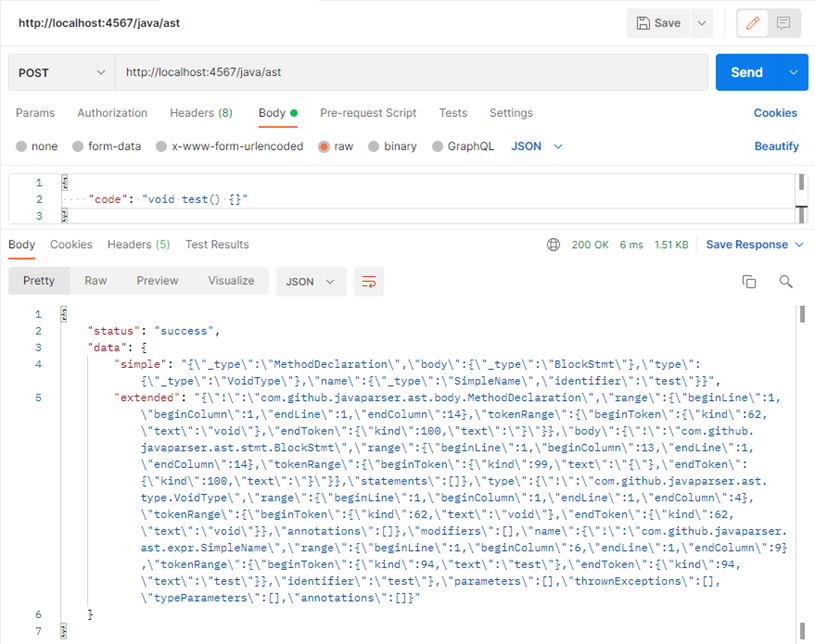
\includegraphics [scale=0.65] {my_folder/images/my/20}
	\caption{Тестирование сервера визуализатора} 
	\label{fig:20}  
\end{figure}

В запросе мы подаем на вход исходный код, который требуется парсить, а на выходе получаем результат работы JavaParser в двух видах: simple (который потребуется для рисования) и extended (с указанием связей с исходным кодом и прочей информацией). Исходя из результата тестирования можно сделать вывод, что сервер работает так, как надо.
\section{Тестирование клиента} \label{ch6:sec2}
Тестирование клиента проводится вручную в таких браузерах, как Яндекс Браузер, Google Chrome, Firefox, Opera, Edge за счет анализа ряда методов, написанных на Java для каждой модели. Ниже приведены рисунки с результатом работы визуализатора для одного из методов (sumOdd, упомянутый в первой главе) в каждом браузере.

\begin{figure}[h]
	\center
	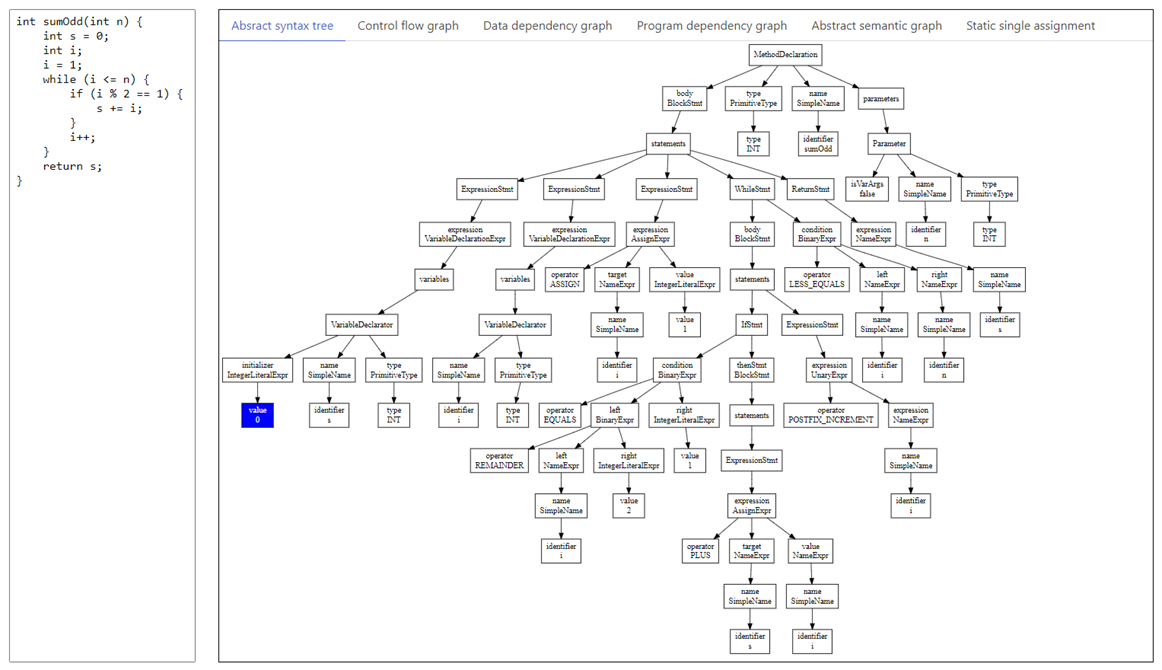
\includegraphics [scale=0.5] {my_folder/images/my/21}
	\caption{Построенное AST в браузере Edge}
	\label{fig:21}
\end{figure}

\begin{figure}[h]
	\center
	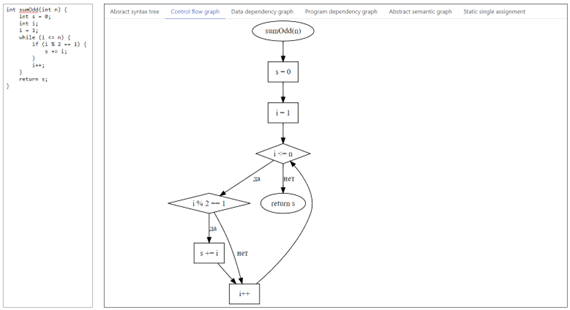
\includegraphics [scale=0.6] {my_folder/images/my/22}
	\caption{Построенный CFG в Яндекс браузере}
	\label{fig:22}
\end{figure}

Как можно увидеть на рисунке 6.2, в дереве присутствуют только семантически значимые узлы. Если блок подсвечен синим цветом, то это означает, что все его наследники скрыты.

На построенном CFG используются стандартные формы для обозначения узлов: эллипс для обозначения начала или конца, прямоугольник для обычных операторов, ромб для узлов принятия решений. Рёбра, выходящие из узлов принятия решений, имеют обозначения, дающие понять, по какому ребру переходить в случае, если условие истинно, а по какому в случае, если ложно.

\begin{figure}[h]
	\center
	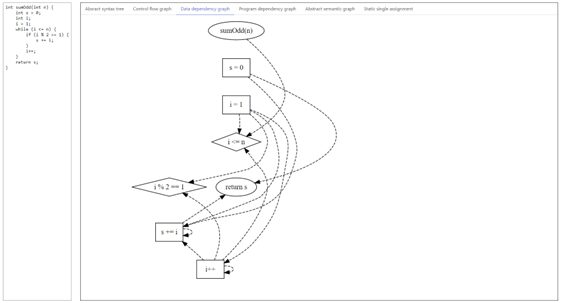
\includegraphics [scale=0.48] {my_folder/images/my/23}
	\caption{Построенный DDG в браузере Chrome}
	\label{fig:23}
\end{figure}

\begin{figure}[h]
	\center
	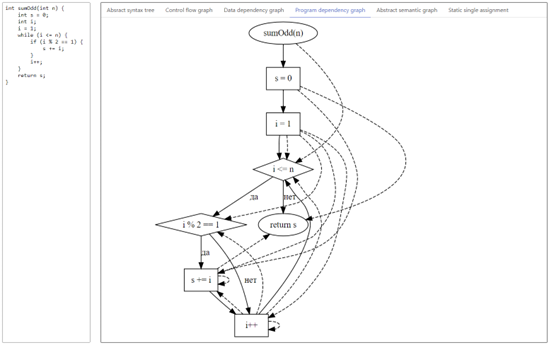
\includegraphics [scale=0.65] {my_folder/images/my/24}
	\caption{Построенный PDG в браузере Opera}
	\label{fig:24}
\end{figure}

\begin{figure}[h]
	\center
	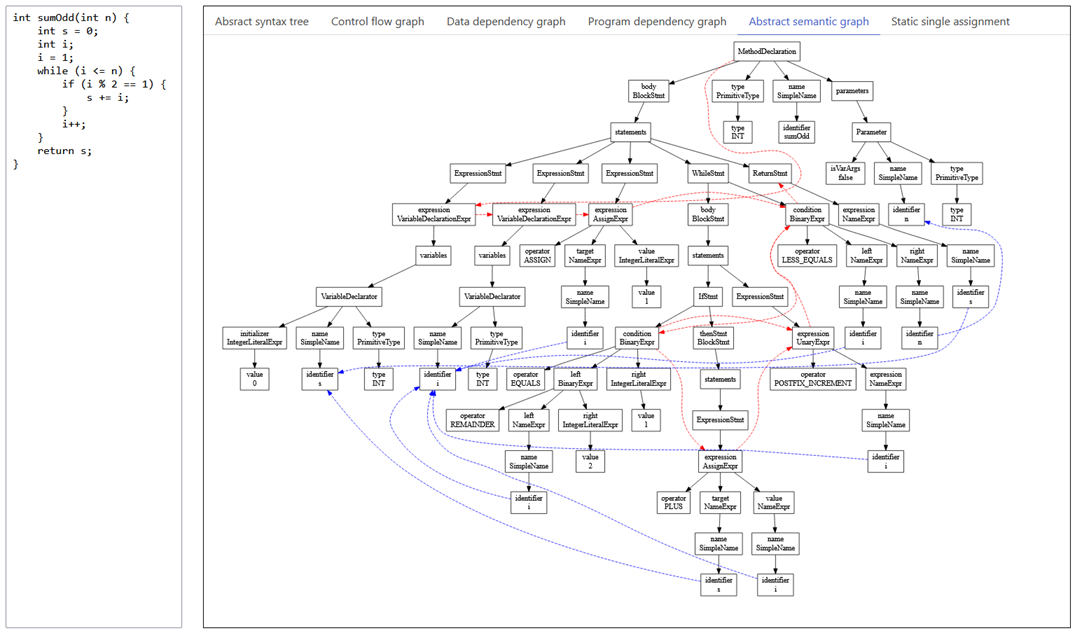
\includegraphics [scale=0.55] {my_folder/images/my/25}
	\caption{Построенный ASG в браузере Firefox}
	\label{fig:25}
\end{figure}

На рисунке 6.6 видно, что при отрисовке ребра между соседними инструкциями для наглядности обозначаются красными пунктирными стрелками, а рёбра между объявлениями и использованием переменных пунктирными синими.

\begin{figure}[h]
	\center
	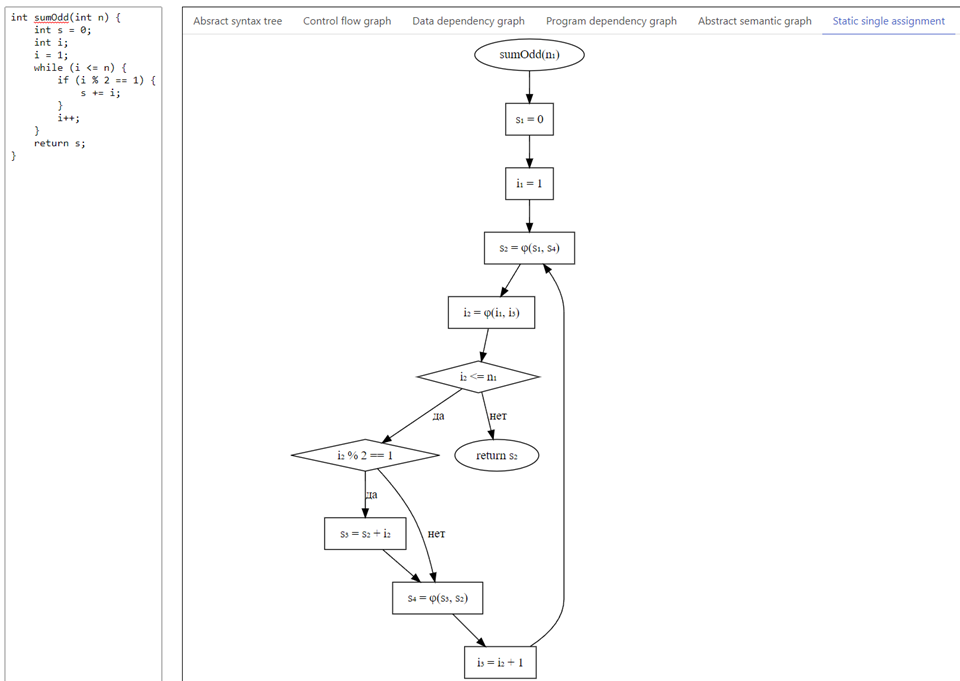
\includegraphics [scale=0.5] {my_folder/images/my/26}
	\caption{Построенное SSA в Яндекс браузере}
	\label{fig:26}
\end{figure}

\begin{figure}[h]
	\center
	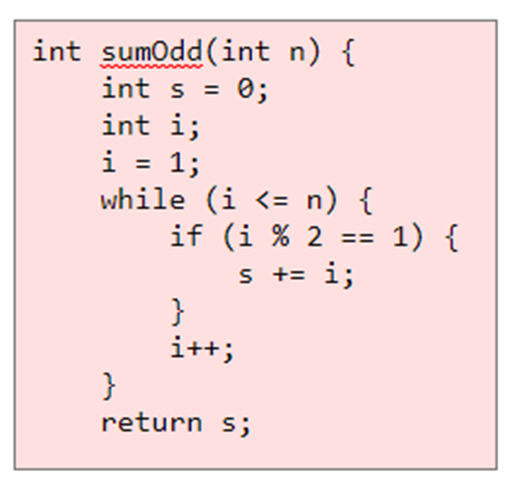
\includegraphics [scale=0.5] {my_folder/images/my/27}
	\caption{Неправильно введенный код}
	\label{fig:27}
\end{figure}

Если код написан неверно, то интерфейс подсвечивается красным цветом и отрисовка и изменение уже нарисованной модели не происходит.\newpage
\section{Выводы по главе} \label{ch6:sec3}
В данной главе рассмотрено тестирование сервера и клиента визуализатора. Сервер протестирован с помощью утилиты Postman, а клиент тестировался в разных браузерах для разных методов, написанных на Java. В отчете приведен один из них. Из результатов тестирования можно сделать вывод, что сервис работает, так как надо.
\newpage               % Глава 6
\ContinueChapterEnd % завершить размещение глав <<подряд>>
%% Завершение основной части

\chapter*{Заключение} \label{ch-conclusion}
\addcontentsline{toc}{chapter}{Заключение}	% в оглавление 
В рамках выпускной квалификационной работы был разработан сервис интерактивной визуализации моделей программ, как средство для улучшения понимания устройства абстрактного синтаксического дерева, графа потока управления, графа зависимостей по данным, графа зависимости программы, абстрактного семантического графа и представления на основе однократного статического присваивания. 
Сперва были рассмотрены аналоги, их плюсы и минусы. Исходя из обзора был сделан вывод, что на данным момент не существует универсального и хорошего продукта, у всех есть какие-либо недостатки, так же не существует ни одного сервиса, который мог бы построить несколько заявленных моделей. После разбора были получены требования к системе, выбрана библиотека для рисования, парсер кода и фреймворк для сервера и клиента и была описана разработка. Итоговая версия визуализатора имеет клиент-серверную архитектуру, сервер написан на языке программирования Java, использует парсер JavaParser и фреймворк Spark. Клиент же написан на языке программирования JavaScript с использованием фреймворка Vue.js, библиотекой axios для сетевых запросов, фреймворка bulma для оформления интерфейса и использует библиотеку d3-graphviz для визуализации моделей.
Сервис был протестирован за счет анализа ряда методов, написанных на Java. Ожидаемые деревья и графы совпали с теми, которые рисует визуализатор и сейчас им можно пользоваться в образовательных целях. В будущем планируется добавление других языков программирования и расширение функционала.
\newpage        	 % Заключение

%% Наличие следующих перечней не исключает расшифровку сокращения и условного обозначения при первом упоминании в тексте!
%\input{my_folder/acronyms}		         % Необязательная рубрика! Список сокращений и условных обозначений

%\input{my_folder/dictionary}    		 % Необязательная рубрика! Словарь терминов
% По порядку после Списка сокращений и условных обозначений, если есть.	


%%% Не мянять - Do not modify
%%
%%
\clearpage                                  % В том числе гарантирует, что список литературы в оглавлении будет с правильным номером страницы
%\hypersetup{ urlcolor=black }               % Ссылки делаем чёрными
%\providecommand*{\BibDash}{}                % В стилях ugost2008 отключаем использование тире как разделителя 
\urlstyle{rm}                               % ссылки URL обычным шрифтом
%\ifdefmacro{\microtypesetup}{\microtypesetup{protrusion=false}}{} % не рекомендуется применять пакет микротипографики к автоматически генерируемому списку литературы
%\newcommand{\fullbibtitle}{Список литературы} % (ГОСТ Р 7.0.11-2011, 4)
%\insertbibliofull  
%\noindent
%\begin{group}
\chapter*{Список использованных источников}
\label{references}
\addcontentsline{toc}{chapter}{Список использованных источников}	% в оглавление 
\printbibliography[env=SSTfirst]                         % Подключаем Bib-базы
1. Глухих М.И., Ицыксон В.М. Программная инженерия. Обеспечение качества программных средств методами статического анализа. Учебное пособие. СПб.: Изд-во Политехн. ун-та. 2011. – 150 с.

2. Кларк Э.М. Верификация моделей программ. Model Checking [пер. с англ.] / Э. М. Кларк, О. Грамберг, Д. Пелед. – М.: МЦНМО, 2002. – 416 c.

3. Синицын С.В. Верификация программного обеспечения / С.В. Синицын, Н.Ю. Налютин. – М: «Интернет-университет информационных технологий – ИНТУИТ.ру», 2008. – 358 с.

4. Bulma official website. - URL: https://bulma.io/ (online; accessed: 13.04.2022).

5. Graphviz DOT rendering and animated transitions using D3. - URL: https://github.com/magjac/d3-graphviz (online; accessed: 13.02.2022).

6. Java documentation, Electronic resourse, Oracle. - URL: https://docs.oracle.com\\/en/java (online; accessed: 24.02.2022).

7. JavaParser official website. - URL: https://javaparser.org (online; accessed: 12.02.2022).

8. Nielson F. Principles of Program Analysis : Corr. 2nd printing / Flemming Nielson, Hanne R. Nielson, Chris Hankin. - Berlin [etc.]: Springer, 2005. - XXI, 452 p., 56 illus. - ISBN 978-3-540-65410-0.

9. Postman official website. - URL: https://www.postman.com/ (online; accessed: 11.05.2022).

10. React Official Documentation, Electronic resource, Facebook. - URL: https://reactjs.org/docs/getting-started.html (online;accessed: 31.05.2022).

11. Spark Framework tutorials. - URL: https://sparktutorials.github.io/ (online; accessed: 04.02.2022).

12. Vue.js official website. - URL: https://ru.vuejs.org/ (online; accessed: 13.04.2022).




%\ifdefmacro{\microtypesetup}{\microtypesetup{protrusion=true}}{}
%\urlstyle{tt}                               % возвращаем установки шрифта ссылок URL
%\hypersetup{ urlcolor={urlcolor} }          % Восстанавливаем цвет ссылок



%\urlstyle{rm}                               % ссылки URL обычным шрифтом
%\ifdefmacro{\microtypesetup}{\microtypesetup{protrusion=false}}{} % не рекомендуется применять пакет микротипографики к автоматически генерируемому списку литературы
%\insertbibliofull                           % Подключаем Bib-базы
%\ifdefmacro{\microtypesetup}{\microtypesetup{protrusion=true}}{}
%\urlstyle{tt}                               % возвращаем установки шрифта ссылок URL
		     % Список литературы

% Здесь можно поместить список иллюстративного материала

\appendix % не редактировать / keep unmodified


\chapter{Репозитории с исходным кодом клиента и сервера визуализатора}\label{appendix-MikTeX-TexStudio} % Заголовок

Исходный код клиента:\\
https://github.com/Resident0014/visualizer\_front\\

Исходный код сервера:\\
https://github.com/Resident0014/visualizer\_server\\			     % Приложение 1
\chapter{Исходный код клиентской части визуализатора}\label{appendix-MikTeX-TexStudio}							%

\lstset{
frame=single,
numbersep = 5pt,
stepnumber = 1
}

\begin{flushright}
Листинг П2.1. Содержимое файла ast.js
\end{flushright}

\begin{lstlisting}
export const getData = (tree) => {
  const nodes = []
  const edges = []
  const hierarchy = {}

  const addNode = (node, from) => {
    node.idx = nodes.push(node) - 1
    node.hidden = false
    node.from = from
    if (!hierarchy[from]) {
      hierarchy[from] = []
    }
    hierarchy[from].push(node.idx)
    edges.push({ from, to: node.idx, hidden: false })
    return node.idx
  }

  const parseNode = (node, edgeFrom = null, name = null) => {
    if (Array.isArray(node)) {
      const parentIdx = addNode({ label: name }, edgeFrom)
      for (const subNode of node) {
        parseNode(subNode, parentIdx)
      }
    } else if (typeof node === 'object') {
      const { _type, ...fields } = node
      const parentIdx = addNode({
        label: name ? `${name}\n${_type}` : _type,
        orig: node
      }, edgeFrom)
      for (const [fieldName, subNode] of Object.entries(fields)) {
        parseNode(subNode, parentIdx, fieldName)
      }
    } else {
      addNode({ label: `${name}\n${node}` }, edgeFrom)
    }
  }

  parseNode(tree)

  edges.shift()

  return { nodes, edges, hierarchy }
}

export const dataToAstDigraph = (nodes, edges) => {
  const lines = []
  for (const [i, node] of nodes.entries()) {
    if (node.hidden) continue
    const attrs = [
      `label="${escapeQuotes(node.label)}"`,
      'shape="box"'
    ]
    if (node.clicked) {
      attrs.push('style="filled", fillcolor="blue", fontcolor="white"')
    }
    lines.push(`n${i} [${attrs.join(',')}]`)
  }
  for (const edge of edges) {
    if (edge.hidden) continue
    lines.push(`n${edge.from} -> n${edge.to}`)
  }
  return `digraph { ${lines.join(';')} }`
}
\end{lstlisting}

\begin{flushright}
Листинг П2.2. Содержимое файла cfg.js
\end{flushright}

\begin{lstlisting}
import { getType, getCodeGetterByElement, escapeQuotes } from './_common'

export const getCfgData = (code, tree) => {
  const getCode = getCodeGetterByElement(code)

  const nodes = []
  const edges = []

  const operators = {
    PLUS: '+',
    MINUS: '-',
    MULTIPLY: '*',
    DIVIDE: '/',
    REMAINDER: '%',
    XOR: '^',
    BINARY_AND: '&',
    BINARY_OR: '|',
    ASSIGN: ''
  }

  const edgesQueue = []
  const loopStack = []
  const addSimpleNode = (node) => {
    const idx = nodes.push(node) - 1
    do {
      const e = edgesQueue.shift()
      e.to = idx
      edges.push(e)
    } while (edgesQueue.length)
    edgesQueue.push({
      from: idx, to: null, type: 'simple'
    })
    return idx
  }

  const addItem = (item) => {
    const adder = addItemByType[getType(item['!'])]
    if (adder) {
      adder(item)
    } else {
      addSimpleNode({
        type: 'statement',
        label: `${getCode(item)}`,
        elem: item
      })
    }
  }

  const addItemByType = {
    MethodDeclaration: (m) => {
      const params = m.parameters.map(p => p.name.identifier).join(', ')
      const idx = nodes.push({
        type: 'method',
        label: `${m.name.identifier}(${params})`,
        elem: m
      }) - 1
      edgesQueue.push({
        from: idx, to: null, type: 'simple'
      })
      addItem(m.body)
    },
    ExpressionStmt: (st) => {
      addItem(st.expression)
    },
    VariableDeclarationExpr: (expr) => {
      for (const v of expr.variables) {
        if (v.initializer) {
          addSimpleNode({
            type: 'statement',
            label: `${v.name.identifier} = ${getCode(v.initializer)}`,
            elem: v
          })
        }
      }
    },
    AssignExpr: (expr) => {
      addSimpleNode({
        type: 'statement',
        label: `${getCode(expr.target)} ${operators[expr.operator]}= ${getCode(expr.value)}`,
        elem: expr
      })
    },
    BlockStmt: (st) => {
      for (const statement of st.statements) {
        addItem(statement)
      }
    },
    WhileStmt: (st) => {
      const idx = addSimpleNode({
        type: 'condition',
        label: `${getCode(st.condition)}`,
        elem: st.condition
      })
      edgesQueue[0].type = 'trueBranch'
      const loop = {
        breaks: [],
        continues: []
      }
      loopStack.push(loop)
      addItem(st.body)
      for (const edge of loop.continues) {
        edgesQueue.push(edge)
      }
      while (edgesQueue.length) {
        const e = edgesQueue.shift()
        e.to = idx
        edges.push(e)
      }
      edgesQueue.push({
        from: idx, to: null, type: 'falseBranch'
      })
      for (const edge of loop.breaks) {
        edgesQueue.push(edge)
      }
      loopStack.pop()
    },
    ForStmt: (forSt) => {
      for (const st of forSt.initialization) {
        addItem(st)
      }
      const idx = addSimpleNode({
        type: 'condition',
        label: `${forSt.compare ? getCode(forSt.compare) : 'true'}`,
        elem: forSt.compare
      })
      edgesQueue[0].type = 'trueBranch'
      const loop = {
        breaks: [],
        continues: []
      }
      loopStack.push(loop)
      addItem(forSt.body)
      for (const edge of loop.continues) {
        edgesQueue.push(edge)
      }
      for (const st of forSt.update) {
        addItem(st)
      }
      while (edgesQueue.length) {
        const e = edgesQueue.shift()
        e.to = idx
        edges.push(e)
      }
      edgesQueue.push({
        from: idx, to: null, type: 'falseBranch'
      })
      for (const edge of loop.breaks) {
        edgesQueue.push(edge)
      }
      loopStack.pop()
    },
    IfStmt: (st) => {
      const idx = addSimpleNode({
        type: 'condition',
        label: `${getCode(st.condition)}`,
        elem: st.condition
      })
      edgesQueue[0].type = 'trueBranch'
      addItem(st.thenStmt)
      const thenEdges = edgesQueue.splice(0, edgesQueue.length)
      edgesQueue.push({
        from: idx, to: null, type: 'falseBranch'
      })
      if (st.elseStmt) {
        addItem(st.elseStmt)
      }
      edgesQueue.push(...thenEdges)
    },
    ReturnStmt: (st) => {
      addSimpleNode({
        type: 'return',
        label: `return ${getCode(st.expression)}`,
        elem: st
      })
      while (edgesQueue.length) {
        edgesQueue.pop()
      }
    },
    BreakStmt: () => {
      const { breaks } = loopStack[loopStack.length - 1]
      while (edgesQueue.length) {
        breaks.push(edgesQueue.shift())
      }
    },
    ContinueStmt: () => {
      const { continues } = loopStack[loopStack.length - 1]
      while (edgesQueue.length) {
        continues.push(edgesQueue.shift())
      }
    }
  }

  addItem(tree)

  return { nodes, edges }
}

export const cfgDataToDigraph = (cfgData) => {
  const lines = []
  for (const [i, node] of cfgData.nodes.entries()) {
    let shape
    if (node.type === 'method' || node.type === 'return') {
      shape = 'ellipse'
    } else if (node.type === 'statement') {
      shape = 'box'
    } else if (node.type === 'condition') {
      shape = 'diamond'
    }
    lines.push(`n${i} [label="${escapeQuotes(node.label)}", shape="${shape}"]`)
  }
  for (const edge of cfgData.edges) {
    let line = `n${edge.from} -> n${edge.to}`
    const attrs = []
    if (edge.type === 'trueBranch') {
      attrs.push('label="да"')
    }
    if (edge.type === 'falseBranch') {
      attrs.push('label="нет"')
    }
    if (attrs.length) {
      line += ` [${attrs.join(' ')}]`
    }
    lines.push(line)
  }
  return `digraph { ${lines.join(';')} }`
}
\end{lstlisting}

\begin{flushright}
Листинг П2.3. Содержимое файла ddg-pdg.js
\end{flushright}

\begin{lstlisting}
import { getType, escapeQuotes } from './_common'
import { getCfgData } from './cfg'

const getNodeReadVariables = (node) => {
  const addItem = (item) => {
    const adder = addItemByType[getType(item['!'])]
    if (adder) {
      adder(item)
    }
  }
  const addItemByType = {
    ExpressionStmt: (st) => {
      addItem(st.expression)
    },
    VariableDeclarationExpr: (expr) => {
      for (const v of expr.variables) {
        addItem(v)
      }
    },
    VariableDeclarator: (expr) => {
      if (expr.initializer) {
        addItem(expr.initializer)
      }
    },
    AssignExpr: (expr) => {
      if (expr.operator !== 'ASSIGN') {
        addItem(expr.target)
      }
      addItem(expr.value)
    },
    ReturnStmt: (st) => {
      addItem(st.expression)
    },
    MethodCallExpr: (expr) => {
      for (const arg of expr.arguments) {
        addItem(arg)
      }
    },
    BinaryExpr: (expr) => {
      addItem(expr.left)
      addItem(expr.right)
    },
    UnaryExpr: (expr) => {
      addItem(expr.expression)
    },
    ArrayCreationExpr: (expr) => {
      for (const level of expr.levels) {
        addItem(level)
      }
    },
    ArrayCreationLevel: (expr) => {
      addItem(expr.dimension)
    },
    FieldAccessExpr: (expr) => {
      addItem(expr.scope)
    },
    ArrayAccessExpr: (expr) => {
      addItem(expr.name)
      addItem(expr.index)
    },
    EnclosedExpr: (expr) => {
      addItem(expr.inner)
    },
    NameExpr: (expr) => {
      addItem(expr.name)
    },
    SimpleName: (name) => {
      set.add(name.identifier)
    }
  }
  const set = new Set()
  addItem(node.elem)
  return set
}
const getNodeWriteVariables = (node) => {
  const addItem = (item) => {
    const adder = addItemByType[getType(item['!'])]
    if (adder) {
      adder(item)
    }
  }
  const addItemByType = {
    MethodDeclaration: (m) => {
      for (const param of m.parameters) {
        addItem(param.name)
      }
    },
    ExpressionStmt: (st) => {
      addItem(st.expression)
    },
    VariableDeclarationExpr: (expr) => {
      for (const v of expr.variables) {
        addItem(v)
      }
    },
    VariableDeclarator: (expr) => {
      if (expr.initializer) {
        addItem(expr.name)
      }
    },
    AssignExpr: (expr) => {
      addItem(expr.target)
    },
    UnaryExpr: (expr) => {
      addItem(expr.expression)
    },
    NameExpr: (expr) => {
      addItem(expr.name)
    },
    SimpleName: (name) => {
      set.add(name.identifier)
    }
  }
  const set = new Set()
  addItem(node.elem)
  return set
}

const setVarContext = (nodes, from, vars) => {
  let changed = false
  for (const [v, nodeIdx] of Object.entries(vars)) {
    let w = nodes[from].varContext[v]
    if (!w) {
      w = nodes[from].varContext[v] = new Set()
    }
    if (!w.has(nodeIdx)) {
      w.add(nodeIdx)
      changed = true
    }
  }
  nodes[from].visited = true
  for (const v of nodes[from].writeVariables) {
    vars[v] = from
  }
  for (const to of nodes[from].jumps) {
    if (!nodes[to].visited || changed) {
      setVarContext(nodes, to, { ...vars })
    }
  }
}

const getDeps = (nodes) => {
  const deps = []
  for (const [to, node] of nodes.entries()) {
    for (const v of node.readVariables) {
      for (const from of node.varContext[v]) {
        deps.push({ from, to })
      }
    }
  }
  return deps
}

const getData = (code, tree) => {
  const { nodes, edges } = getCfgData(code, tree)
  for (const node of nodes) {
    node.jumps = []
    node.varContext = {}
    node.readVariables = getNodeReadVariables(node)
    node.writeVariables = getNodeWriteVariables(node)
  }
  for (const edge of edges) {
    nodes[edge.from].jumps.push(edge.to)
  }
  setVarContext(nodes, 0, {})
  const deps = getDeps(nodes)
  return { nodes, edges, deps }
}

const dataToDigraph = (code, tree, defaultEdgeAttr) => {
  const data = getData(code, tree)
  const lines = []
  for (const [i, node] of data.nodes.entries()) {
    let shape
    if (node.type === 'method' || node.type === 'return') {
      shape = 'ellipse'
    } else if (node.type === 'statement') {
      shape = 'box'
    } else if (node.type === 'condition') {
      shape = 'diamond'
    }
    lines.push(`n${i} [label="${escapeQuotes(node.label)}", shape="${shape}"]`)
  }
  for (const edge of data.edges) {
    let line = `n${edge.from} -> n${edge.to}`
    const attrs = [defaultEdgeAttr]
    if (edge.type === 'trueBranch') {
      attrs.push('label="да"')
    }
    if (edge.type === 'falseBranch') {
      attrs.push('label="нет"')
    }
    line += ` [${attrs.join(' ')}]`
    lines.push(line)
  }
  for (const edge of data.deps) {
    lines.push(`n${edge.from} -> n${edge.to} [style="dashed", constraint=false]`)
  }
  return `digraph { ${lines.join(';')} }`
}

export const dataToDdgDigraph = (code, tree) => {
  return dataToDigraph(code, tree, 'style=invis')
}

export const dataToPdgDigraph = (code, tree) => {
  return dataToDigraph(code, tree, 'style=solid')
}
\end{lstlisting}

\begin{flushright}
Листинг П2.4. Содержимое файла asg.js
\end{flushright}

\begin{lstlisting}
import { getData as getAstData } from './ast'
import { escapeQuotes } from './_common'

const getInstructionEdges = (nodes, tree) => {
  const edges = []
  const nodeMap = new Map()
  for (const node of nodes) {
    if (node.orig) {
      nodeMap.set(node.orig, node.idx)
    }
  }

  const edgesQueue = []
  const loopStack = []
  const addInstructionNode = (idx) => {
    do {
      const e = edgesQueue.shift()
      e.to = idx
      edges.push(e)
    } while (edgesQueue.length)
    edgesQueue.push({
      from: idx, to: null
    })
  }

  const addItem = (item) => {
    const adder = addItemByType[item._type]
    if (adder) {
      adder(item)
    } else {
      addInstructionNode(nodeMap.get(item))
    }
  }

  const addItemByType = {
    MethodDeclaration: (m) => {
      edgesQueue.push({
        from: nodeMap.get(m), to: null
      })
      addItem(m.body)
    },
    ExpressionStmt: (st) => {
      addItem(st.expression)
    },
    BlockStmt: (st) => {
      for (const statement of st.statements) {
        addItem(statement)
      }
    },
    WhileStmt: (st) => {
      const idx = nodeMap.get(st.condition)
      addInstructionNode(idx)
      const loop = {
        breaks: [],
        continues: []
      }
      loopStack.push(loop)
      addItem(st.body)
      for (const edge of loop.continues) {
        edgesQueue.push(edge)
      }
      while (edgesQueue.length) {
        const e = edgesQueue.shift()
        e.to = idx
        edges.push(e)
      }
      edgesQueue.push({
        from: idx, to: null
      })
      for (const edge of loop.breaks) {
        edgesQueue.push(edge)
      }
      loopStack.pop()
    },
    ForStmt: (forSt) => {
      for (const st of forSt.initialization) {
        addItem(st)
      }
      const idx = nodeMap.get(forSt.compare)
      addInstructionNode(idx)
      const loop = {
        breaks: [],
        continues: []
      }
      loopStack.push(loop)
      addItem(forSt.body)
      for (const edge of loop.continues) {
        edgesQueue.push(edge)
      }
      for (const st of forSt.update) {
        addItem(st)
      }
      while (edgesQueue.length) {
        const e = edgesQueue.shift()
        e.to = idx
        edges.push(e)
      }
      edgesQueue.push({
        from: idx, to: null
      })
      for (const edge of loop.breaks) {
        edgesQueue.push(edge)
      }
      loopStack.pop()
    },
    IfStmt: (st) => {
      const idx = nodeMap.get(st.condition)
      addInstructionNode(idx)
      addItem(st.thenStmt)
      const thenEdges = edgesQueue.splice(0, edgesQueue.length)
      edgesQueue.push({
        from: idx, to: null
      })
      if (st.elseStmt) {
        addItem(st.elseStmt)
      }
      edgesQueue.push(...thenEdges)
    },
    ReturnStmt: (st) => {
      addInstructionNode(nodeMap.get(st))
      while (edgesQueue.length) {
        edgesQueue.pop()
      }
    },
    BreakStmt: () => {
      const { breaks } = loopStack[loopStack.length - 1]
      while (edgesQueue.length) {
        breaks.push(edgesQueue.shift())
      }
    },
    ContinueStmt: () => {
      const { continues } = loopStack[loopStack.length - 1]
      while (edgesQueue.length) {
        continues.push(edgesQueue.shift())
      }
    }
  }

  addItem(tree)

  return edges
}

const getVarEdges = (nodes, hierarchy) => {
  const declTypes = ['VariableDeclarator', 'Parameter']
  const useNodeIdxByVar = {}
  const declNodeIdxByVar = {}
  for (const [i, n] of nodes.entries()) {
    if (n.orig && n.orig._type === 'SimpleName') {
      const varName = n.orig.identifier
      const identifierIdx = hierarchy[i][0]
      if (declTypes.includes(nodes[n.from].orig._type)) {
        declNodeIdxByVar[varName] = identifierIdx
      } else {
        if (!useNodeIdxByVar[varName]) {
          useNodeIdxByVar[varName] = []
        }
        useNodeIdxByVar[varName].push(identifierIdx)
      }
    }
  }
  const varEdges = []
  for (const [varName, declIdx] of Object.entries(declNodeIdxByVar)) {
    for (const useIdx of useNodeIdxByVar[varName]) {
      varEdges.push({ from: useIdx, to: declIdx })
    }
  }
  return varEdges
}

export const getAsgData = (tree) => {
  const { nodes, edges, hierarchy } = getAstData(tree)

  const varEdges = getVarEdges(nodes, hierarchy)
  const instrEdges = getInstructionEdges(nodes, tree)

  return { nodes, edges, varEdges, instrEdges }
}

export const dataToAsgDigraph = ({ nodes, edges, varEdges, instrEdges }) => {
  const lines = []
  for (const [i, node] of nodes.entries()) {
    lines.push(`n${i} [label="${escapeQuotes(node.label)}", shape="box"]`)
  }
  for (const edge of edges) {
    lines.push(`n${edge.from} -> n${edge.to}`)
  }
  for (const edge of varEdges) {
    lines.push(`n${edge.from} -> n${edge.to} [style="dashed", constraint=false, color="blue"]`)
  }
  for (const edge of instrEdges) {
    lines.push(`n${edge.from} -> n${edge.to} [style="dashed", constraint=false, color="red"]`)
  }
  return `digraph { ${lines.join(';')} }`
}
\end{lstlisting}
			 	 % Приложение 2
\end{document}



%%% Удачной защиты ВКР! - Good luck on the thesis defense!
%%
%%% Поддержать проект
%%
%% Запросы на добавление / изменение просим писать на следующей странице:
%% https://github.com/ParkhomenkoV/SPbPU-student-thesis-template/issues
%%
%% Список пожеланий в файле шаблона <<TO-DO-list.tex>>
%%
%% Благодарности просим указывать в виде 
%%
%% 1. Добавление <<Звезды>> проекту https://github.com/ParkhomenkoV/SPbPU-student-thesis-template/stargazers
%%
%% 2. Добавления <<Сердечка>> и репоста проекта в социальных сетях:
%%		https://vk.com/latex_polytech 
%%		https://www.fb.com/groups/latex.polytech
%%

%%% Support project
%%
%% Requests on adding / modifications is better to be publishen on the following web-page:
%% https://github.com/ParkhomenkoV/SPbPU-student-thesis-template/issues
%%
%% Wishlist is in the template's file called <<TO-DO-list.tex>>
%%
%% Acknowledgements are better to be done in the form of 
%%
%% 1. Adding <<Star>> to the project https://github.com/ParkhomenkoV/SPbPU-student-thesis-template/stargazers
%%
%% 2. Adding <<Likes>> and Project repost in the social networks:
%%		https://vk.com/latex_polytech 
%%		https://www.fb.com/groups/latex.polytech
%% 

% Check list при передаче ВКР:
% - Количество страниц в Задании 2. Если нет, то комментирование последней строки в my_task.tex
% - Зачистка всех вспомогательных файлов (Clear auxilary files) и компиляция ВКР не менее 3х раз